\chapterimage{tabl_cont4.pdf} % Chapter heading image

\chapter{Power BI}
\section{Introduzione}
\textbf{Power BI} è una piattaforma di Business Intelligence sviluppata da Microsoft, progettata per supportare le aziende nell'analisi dei dati e nell'estrapolazione di informazioni strategiche. Integrando strumenti avanzati di \textit{business analytics}, visualizzazione dei dati e \textit{best practice}, Power BI consente alle organizzazioni di prendere decisioni basate su dati concreti, offrendo un ambiente intuitivo e altamente performante per l'esplorazione e l'interpretazione delle informazioni.  

\begin{figure}[h!]
    \centering
    
\includegraphics[width=0.5\linewidth]{capitolo_4/img4/Power-BI_logo.png}
    \caption{Power BI - Logo}
    \label{fig:PowerBI_logo}
\end{figure}

La piattaforma integra nativamente lo scripting \textit{R}, un linguaggio di programmazione specializzato nell’analisi statistica dei dati, ampliando le capacità analitiche disponibili. Questa integrazione consente agli utenti di sfruttare oggetti visivi avanzati basati su \textit{R} senza necessità di una conoscenza diretta del linguaggio, facilitando l'implementazione di analisi complesse anche per professionisti senza competenze di programmazione avanzate.

\subsection{Caricamento dei dati}
Nel software Power BI è stato necessario utilizzare tre files: \textbf{FAOSTAT\_data\_1-10-2022}, \textbf{Global Data on Sustainable Energy (2000-2020)} e \textbf{FAOSTAT\_data\_11-24-2020}. Quest’ultimo dataset è stato fondamentale poiché contiene informazioni dettagliate sui paesi, tra cui i codici identificativi come \texttt{ISO2 Code} e \texttt{Country Code}. La sua presenza si è resa indispensabile per superare una limitazione di Power BI, che non consente di creare due relazioni attive tra le stesse tabelle. FAOSTAT\_data\_11-24-2020 ha quindi svolto il ruolo di tabella di ponte, permettendo di mantenere la connessione tra i diversi dataset senza compromettere la struttura dei dati.  
Prima di procedere alla creazione delle relazioni, si è reso necessario uniformare i nomi dei paesi presenti nei dataset, operazione eseguita direttamente in Power BI utilizzando la funzione \textit{"Trasforma Dati"}. Questo passaggio ha garantito la corretta corrispondenza tra i valori, evitando problemi di inconsistenza nella fase di analisi. Successivamente, si è passati alla definizione delle relazioni tra le tabelle. Per collegare i dati temporali, è stata creata una \textbf{relazione molti-a-molti} tra FAOSTAT\_data\_1-10-2022 e Global Data on Sustainable Energy (2000-2020) utilizzando la colonna \texttt{Year} presente in entrambi i dataset. Questa connessione ha consentito di analizzare in modo congiunto i dati relativi al cambiamento della temperatura e quelli legati all'energia sostenibile nel periodo 2000-2020.  
Oltre alla relazione basata sugli anni, si è proceduto con la connessione tra i Paesi. In questo caso, è stata stabilita una \textbf{relazione uno-a-molti} tra FAOSTAT\_data\_11-24-2020 e FAOSTAT\_data\_1-10-2022, utilizzando la colonna \texttt{Country} di FAOSTAT\_data\_11-24-2020 e la colonna \texttt{Area} di FAOSTAT\_data\_1-10-2022. Questo collegamento ha permesso di associare correttamente i dati relativi ai cambiamenti di temperatura ai rispettivi Paesi. Analogamente, è stata creata un'ulteriore \textbf{relazione uno-a-molti} tra FAOSTAT\_data\_11-24-2020 e Global Data on Sustainable Energy (2000-2020), mettendo in relazione la colonna \texttt{Country} di FAOSTAT\_data\_11-24-2020 con la colonna \texttt{Entity} di Global Data on Sustainable Energy (2000-2020).  
Grazie a questa struttura relazionale, è stato possibile integrare i dati provenienti dalle diverse fonti mantenendo la loro coerenza e affidabilità. La presenza della tabella di ponte ha consentito di risolvere le limitazioni strutturali di Power BI, garantendo una corretta associazione dei dati senza generare relazioni ambigue o errori di connessione. Questa impostazione ha reso possibile la creazione di dashboard interattive che permettono di analizzare le variazioni di temperatura e i dati relativi all'energia sostenibile in modo dettagliato, confrontando facilmente i valori per ogni paese e anno. La corretta definizione delle relazioni tra i dataset ha quindi svolto un ruolo fondamentale nell’ottenere visualizzazioni accurate e coerenti, facilitando l’interpretazione dei dati e migliorando l’efficacia dell’analisi.
\section{Data Analysis}
Per condurre le analisi proposte, sono state elaborate delle \textbf{Dashboard}, costituite da una raccolta di oggetti visivi che rappresentano graficamente i dati del modello.  

Di seguito, vengono presentate le analisi ottenute dai due dataset esaminati:
\vspace{2mm}
\begin{itemize}
    \item \textbf{CO\textsubscript{2}, energia rinnovabile e clima: il quadro completo}
    \item \textbf{Analisi globale del GDP}
    \item \textbf{Andamento delle emissioni di CO\textsubscript{2} in relazione alla crescita del GDP}
    \item \textbf{Andamento produzione di energia rinnovabile rispetto alla crescita del GDP}
\end{itemize}
\vspace{2mm}

\subsection{CO\textsubscript{2}, energia rinnovabile e clima: il quadro completo}
La Dashboard, illustrata in Figura \ref{fig:6.0}, offre una visione dettagliata e sintetica delle interrelazioni tra la variazione della temperatura globale, le emissioni di CO\textsubscript{2} e l'adozione di energie rinnovabili. Questo strumento consente di esaminare in modo chiaro e immediato come questi fattori si influenzino reciprocamente, fornendo un quadro complesso delle dinamiche ambientali ed energetiche a livello globale.

\begin{figure}[h!]
    \centering
    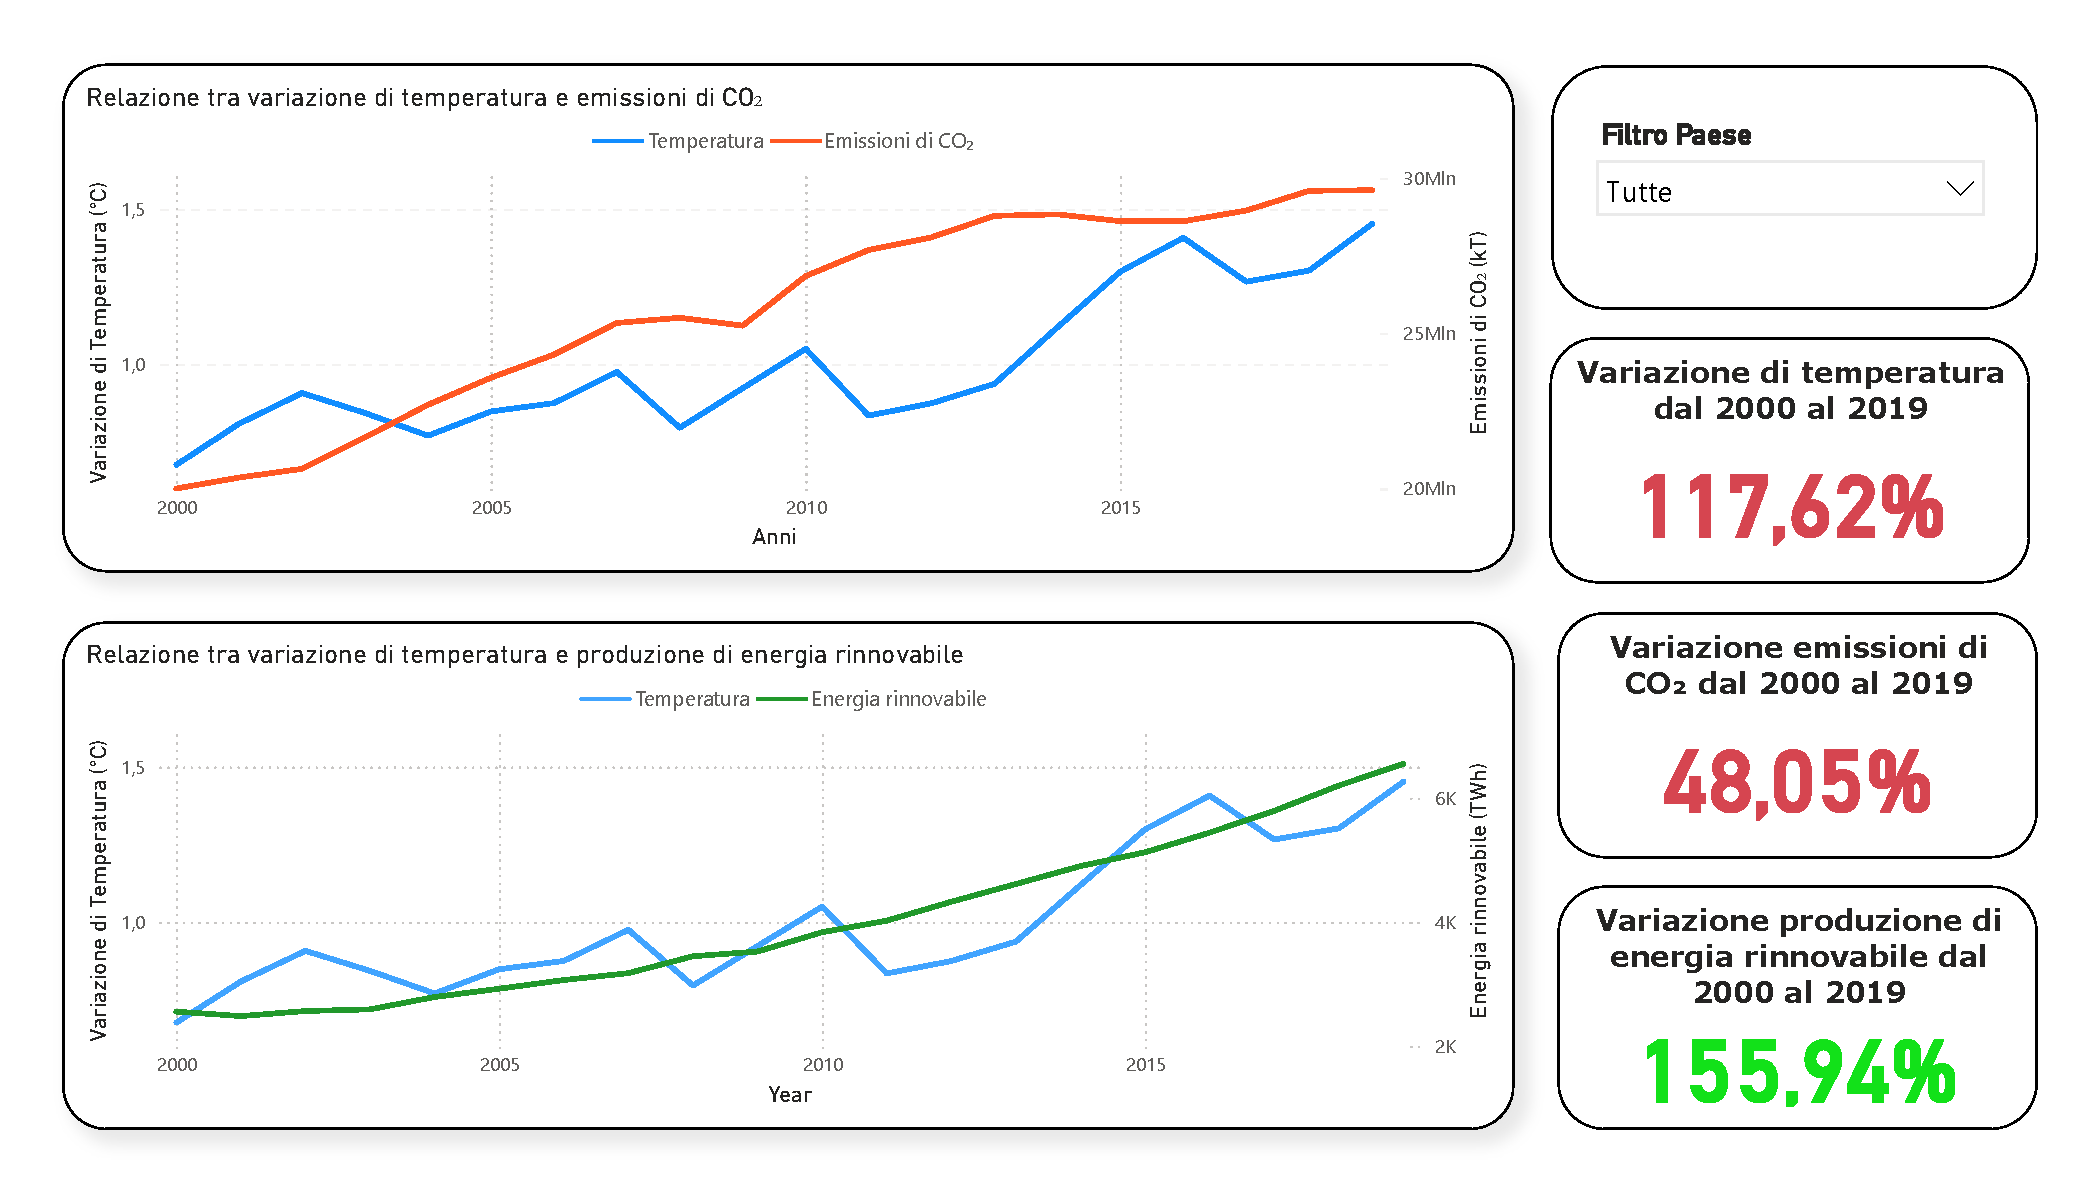
\includegraphics[width=0.98\linewidth]{capitolo_4/img4/AnalisiCO2_temperatura_rinnovabile_casogenerale.pdf}
    \caption{CO\textsubscript{2}, energia rinnovabile e clima: il quadro completo}
    \label{fig:6.0}
\end{figure}

\subsubsection{Struttura della Dashboard}
La Dashboard è progettata per offrire una rappresentazione chiara ed efficace delle dinamiche energetiche e ambientali, combinando diversi strumenti grafici e KPI. La sua struttura è suddivisa in due sezioni principali:
\vspace{2mm}
\begin{itemize}
\item \textit{Parte sinistra}: contiene due visualizzazioni combinate, ciascuna composta da due grafici a linea sovrapposti.
\item \textit{Parte destra}: include tre KPI che sintetizzano in modo immediato i principali indicatori relativi alla temperatura globale, alle emissioni di CO\textsubscript{2} e alla produzione di energia rinnovabile.
\end{itemize}
\vspace{2mm}

Nel dettaglio, i grafici a linee della sezione sinistra presentano le seguenti caratteristiche:
il grafico superiore rappresenta l'andamento delle emissioni di CO\textsubscript{2} nel tempo, espresso in kilotonnellate (kT). Tale visualizzazione consente di individuare trend di crescita o di riduzione delle emissioni di gas serra a livello globale nel periodo analizzato;
Il grafico inferiore mostra, invece, la produzione di energia rinnovabile, misurata in terawattora (TWh), permettendo un confronto diretto tra la crescita delle fonti energetiche sostenibili e le variazioni climatiche.


La sezione destra della Dashboard è composta da tre KPI, che forniscono una sintesi immediata dei dati, facilitandone l'interpretazione:
\vspace{2mm}
\begin{itemize}
\item \textbf{Variazione della temperatura globale dal 2000 al 2019};
\item \textbf{Variazione delle emissioni di CO\textsubscript{2} dal 2000 al 2019};
\item \textbf{Variazione della produzione di energia rinnovabile tra il 2000 e il 2019}.
\end{itemize}
\vspace{2mm}

Un aspetto particolarmente utile della Dashboard è la possibilità di filtrare i dati in base al Paese di interesse. Grazie a questa funzionalità interattiva, l'utente può selezionare uno specifico Stato e visualizzare i grafici e i KPI aggiornati, ottenendo così informazioni personalizzate che rispondono alle proprie esigenze di analisi.

\subsubsection{Obiettivo dell'Analisi}
L'obiettivo primario della Dashboard è fornire una visione chiara e approfondita delle principali tendenze globali legate alle emissioni di CO\textsubscript{2}, alla produzione di energia rinnovabile e ai cambiamenti climatici. L'analisi si concentra sul periodo compreso tra il 2000 e il 2019, evidenziando i principali trend e le correlazioni esistenti tra i diversi fattori.

In particolare, la Dashboard include due grafici fondamentali: \textbf{Relazione tra variazione di temperatura ed emissioni di CO\textsubscript{2}} e \textbf{Relazione tra variazione di temperatura e produzione di energia rinnovabile}. Questi strumenti analitici consentono di osservare la correlazione tra l'incremento della temperatura media globale e due fattori chiave: le emissioni di CO\textsubscript{2} e la produzione di energia da fonti rinnovabili.

L'analisi dei dati suggerisce una chiara correlazione tra l'aumento delle emissioni di CO\textsubscript{2} e l'incremento della temperatura media globale. In particolare, si osserva un trend crescente delle emissioni di gas serra, che sembra accompagnarsi a un incremento progressivo delle temperature. Questo evidenzia l'impatto significativo che le attività umane e il consumo di combustibili fossili hanno sul riscaldamento globale.

Parallelamente, emerge un trend positivo nella produzione di energia rinnovabile, segno che molti Paesi hanno avviato una transizione energetica mirata alla riduzione dell'impatto ambientale. Sebbene questa crescita sia incoraggiante, l'analisi mostra che l'incremento della produzione di energia sostenibile non è ancora sufficiente per compensare completamente le emissioni di gas serra su scala globale.

Come mostrato nella Figura \ref{quadro_completo}, la Dashboard offre la possibilità di filtrare i risultati selezionando specifici Paesi\footnote{I Paesi selezionati per l'analisi sono Cina, Stati Uniti e Italia, scelti in quanto frutto di studi e valutazioni precedenti.}. Questo consente di esaminare in dettaglio le strategie adottate dai vari governi e le loro implicazioni nel contesto della lotta ai cambiamenti climatici.


\begin{figure}[p]
    \centering
    \subfloat[\textbf{Cina}]{%
        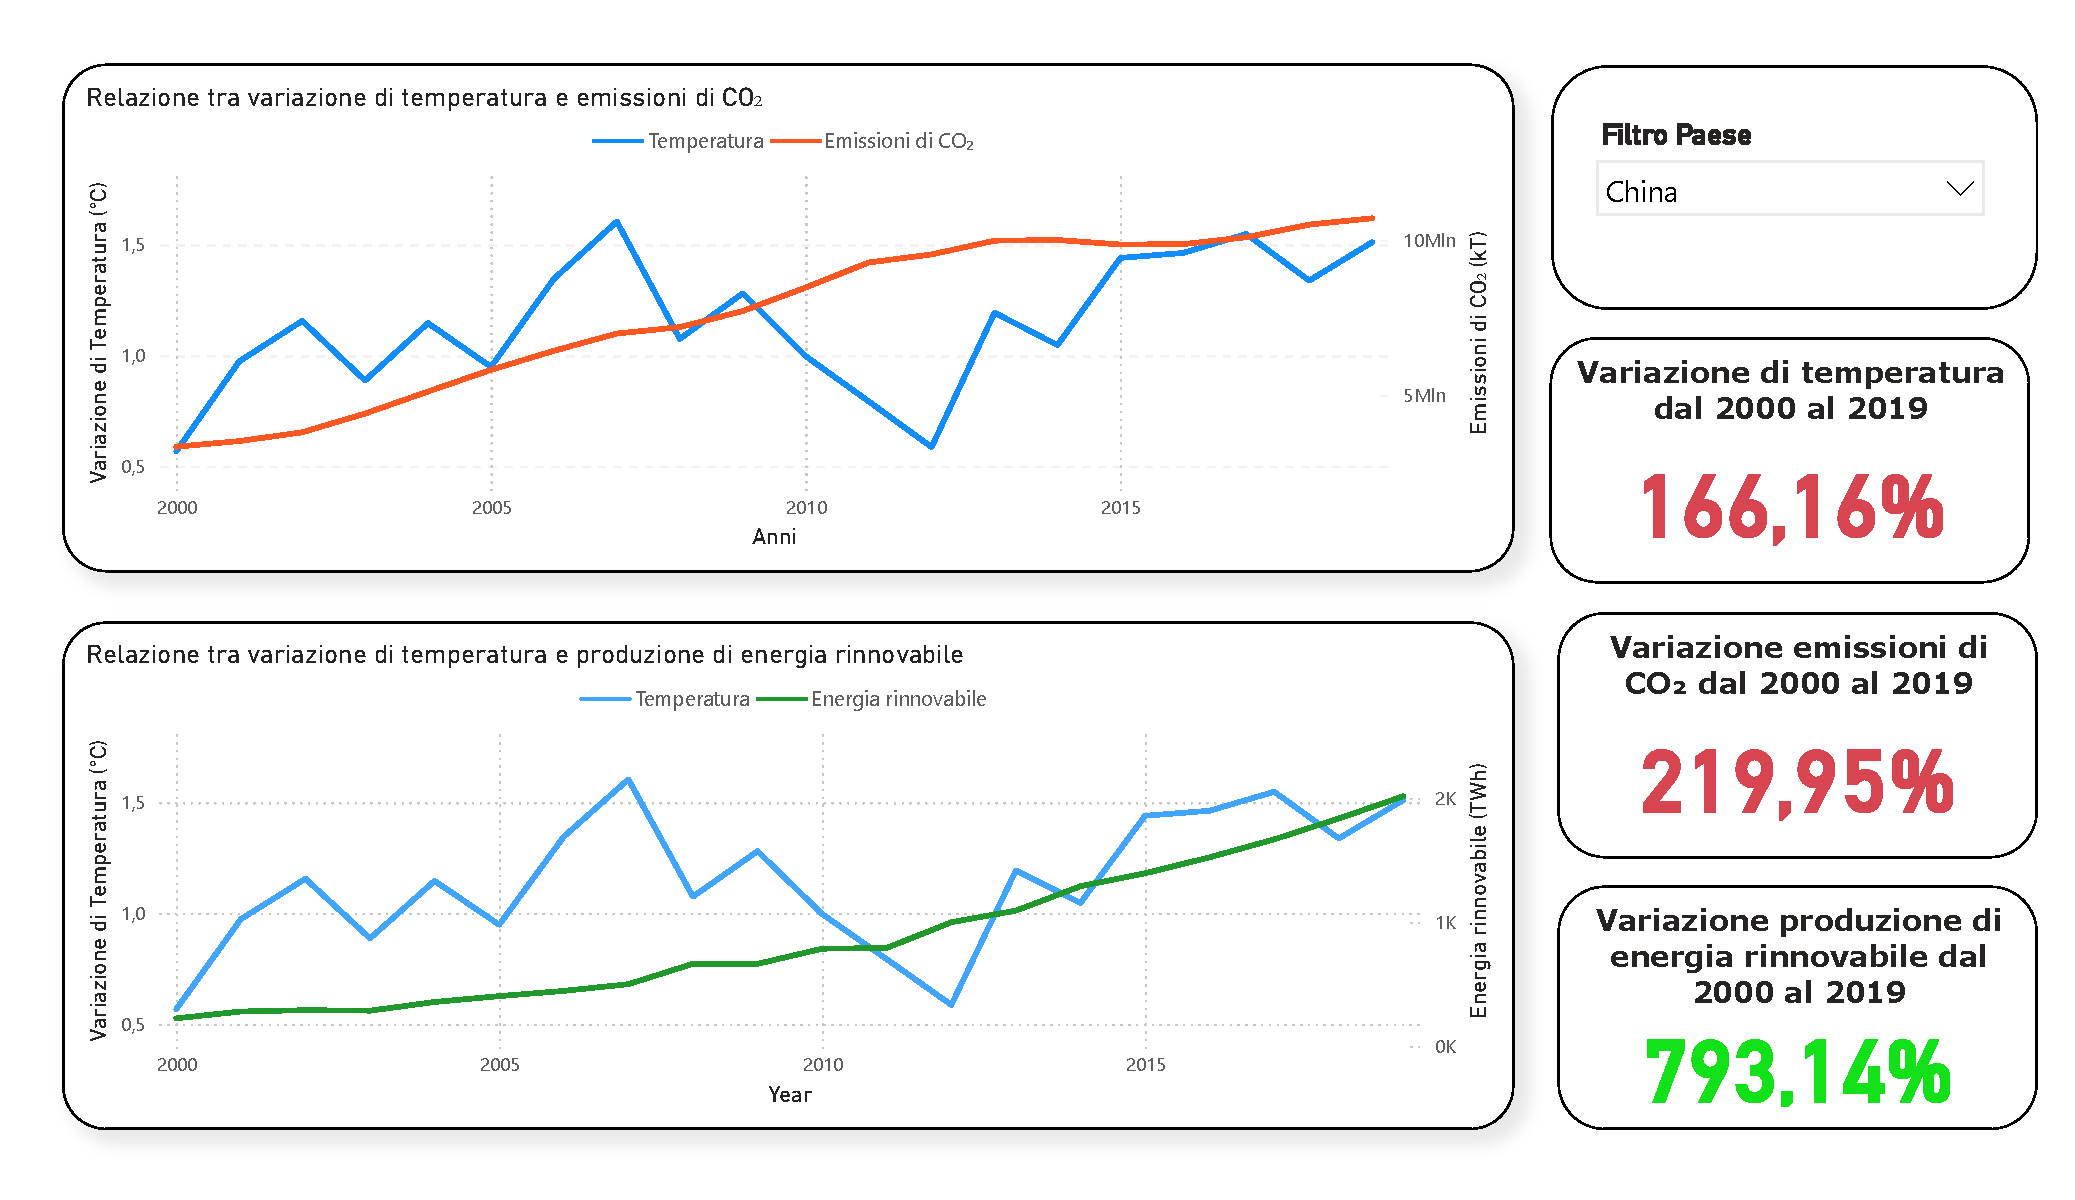
\includegraphics[width=0.8\textwidth]{capitolo_4/img4/AnalisiCO2_temperatura_rinnovabile_Cina.pdf}}\\
    \subfloat[\textbf{USA}]{%
        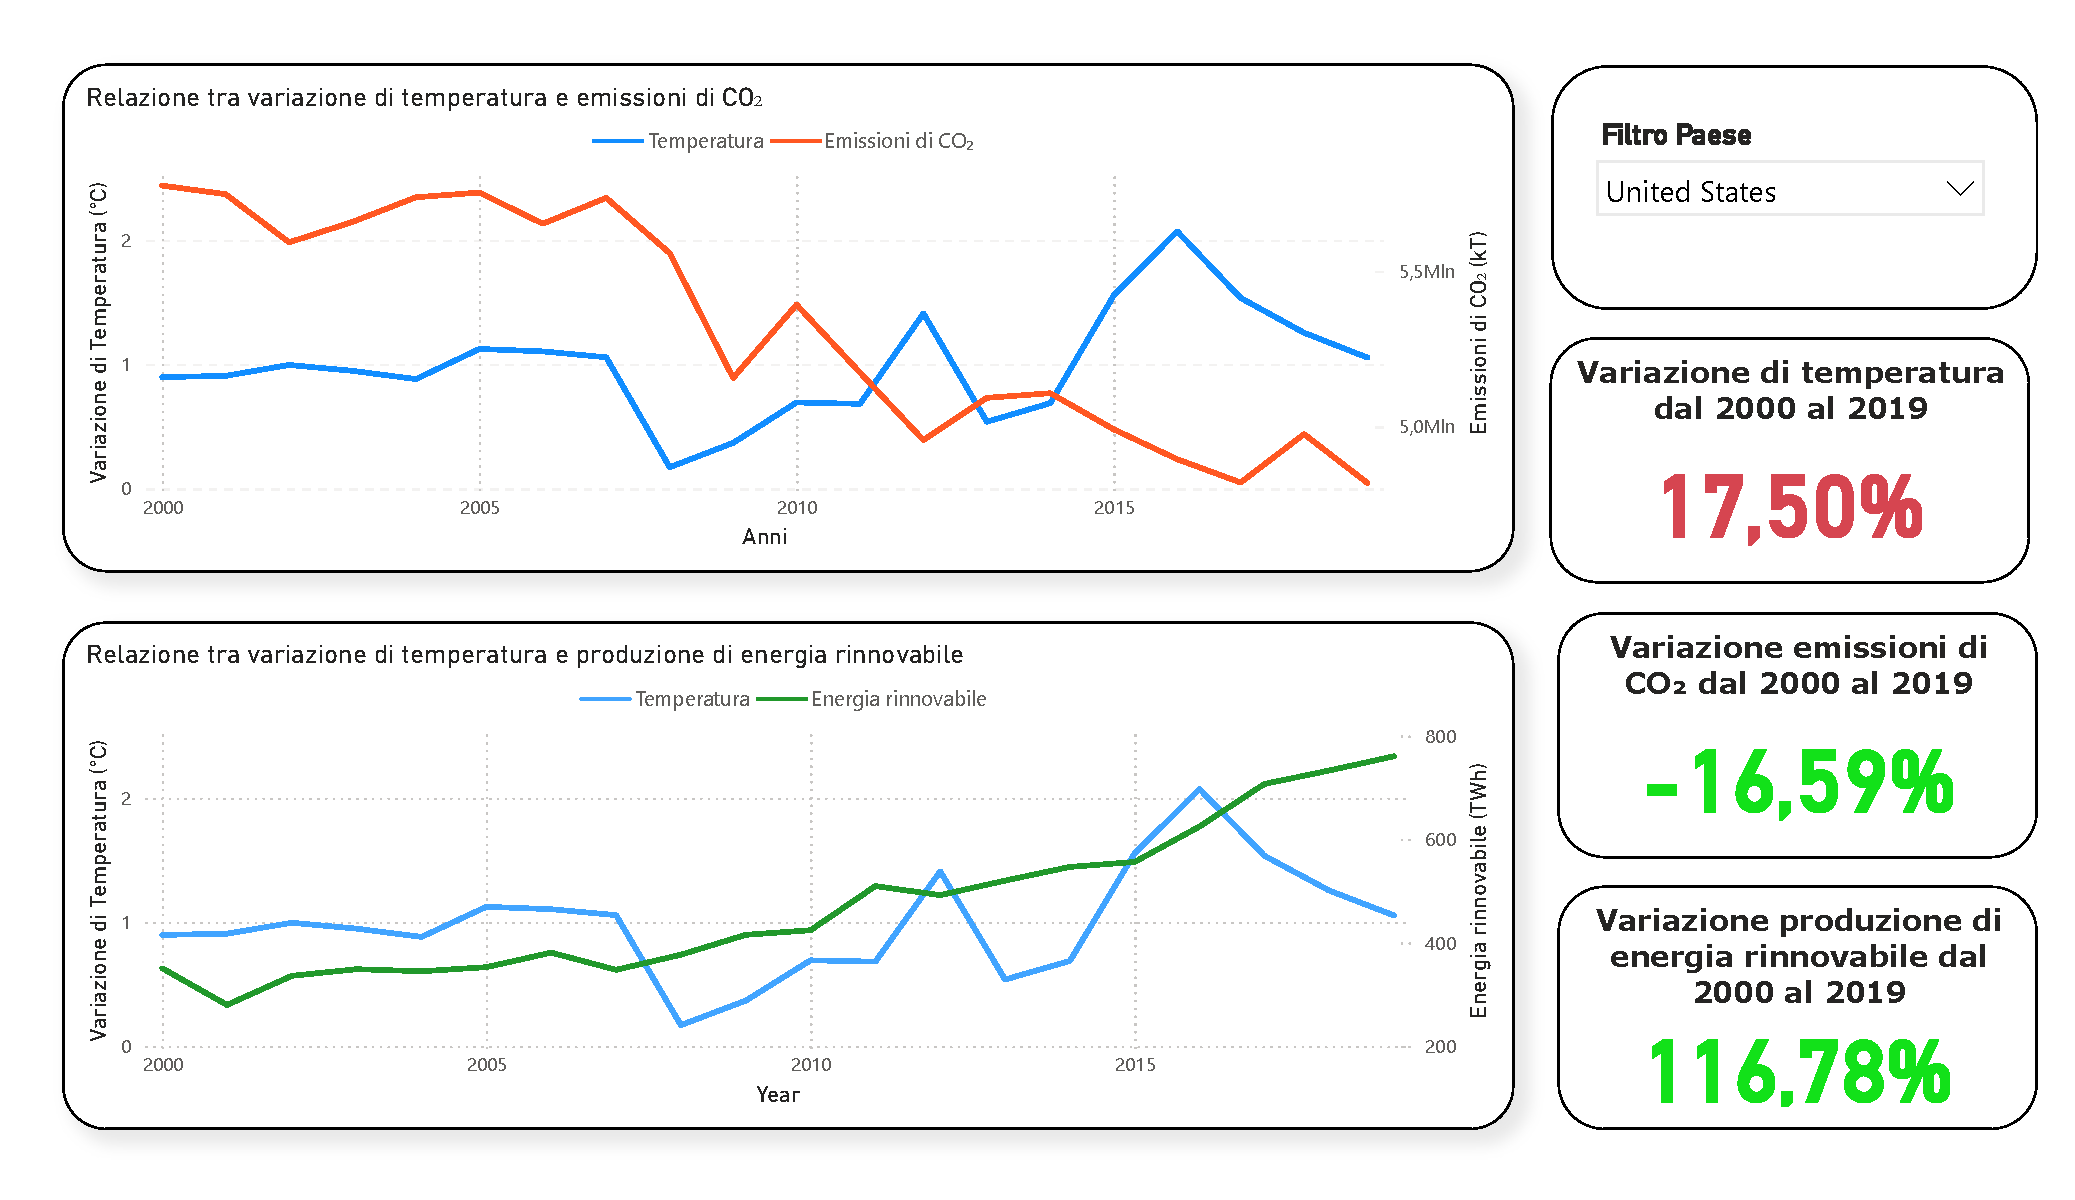
\includegraphics[width=0.8\textwidth]{capitolo_4/img4/AnalisiCO2_temperatura_rinnovabile_USA.pdf}} \\
    \subfloat[\textbf{Italia}]{%
        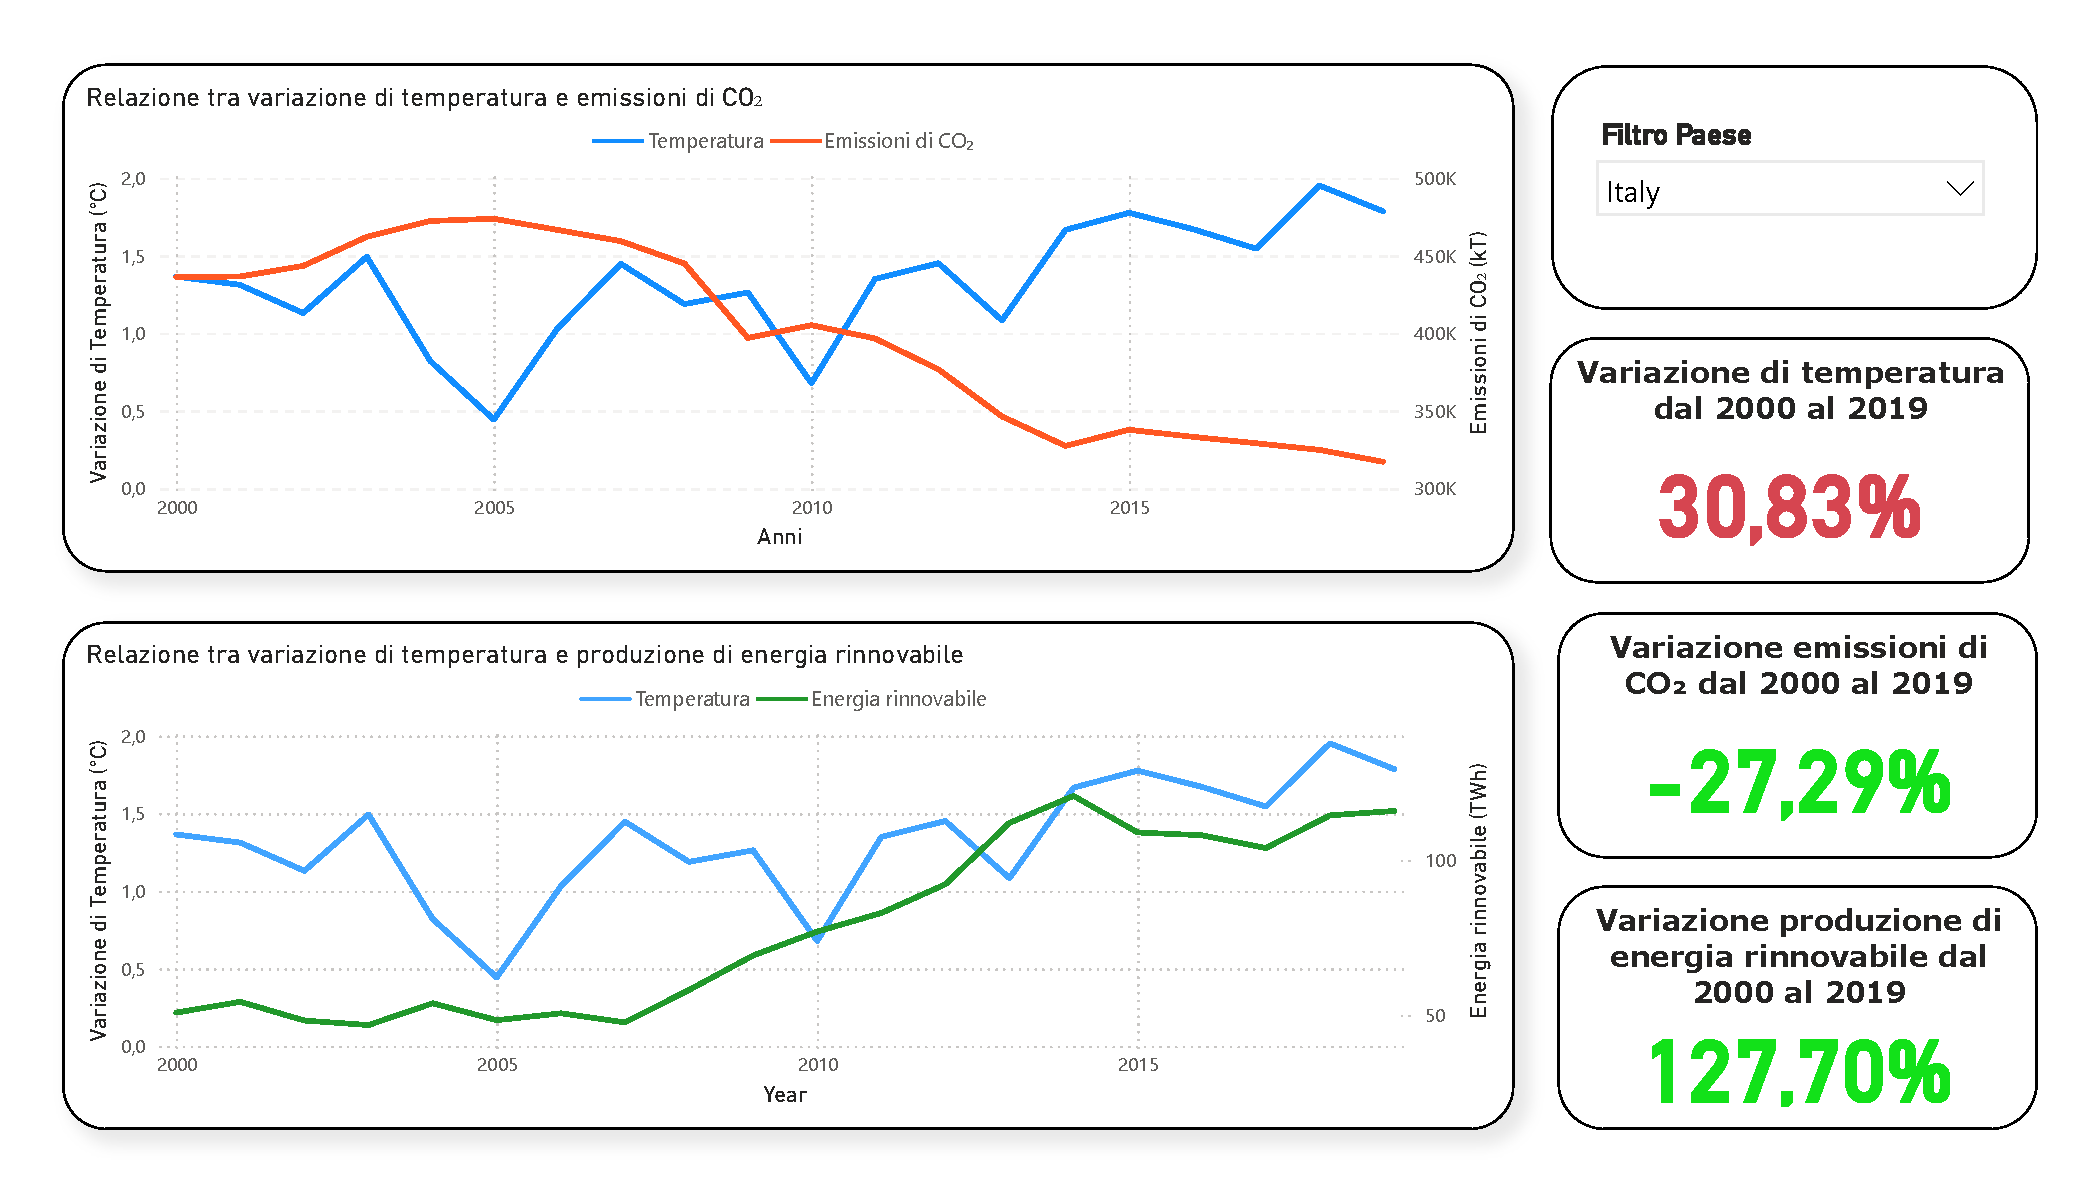
\includegraphics[width=0.8\textwidth]{capitolo_4/img4/AnalisiCO2_temperatura_rinnovabile_Italia.pdf}}

   \caption{CO\textsubscript{2}, energia rinnovabile e clima: il quadro completo - Cina, USA, Italia}
  \label{quadro_completo}
\end{figure}

\newpage
\subsection{Analisi globale del GDP}
La Dashboard, riportata in Figura \ref{fig:GDP_2000}, offre un'analisi dell'economia di diversi Paesi a livello globale, ponendo particolare attenzione a due indicatori fondamentali: il \textbf{Prodotto Interno Lordo (GDP)} e il \textbf{GDP Pro Capite}. Attraverso la rappresentazione congiunta di questi due parametri, è possibile esaminare non solo la dimensione complessiva dell'economia di ciascuna nazione, ma anche il livello medio di ricchezza individuale, consentendo una lettura più completa e significativa delle dinamiche economiche internazionali.

\begin{myoutline}
    \textbf{Nota}: Il \textit{GDP} (\textit{Gross Domestic Product}), corrispondente al \textit{PIL} (\textit{Prodotto Interno Lordo}), è un indicatore economico che misura il valore complessivo di tutti i beni e servizi finali prodotti all'interno di un Paese in un determinato arco temporale, solitamente un anno o un trimestre. Rappresenta uno dei principali parametri per valutare il livello di attività economica e la crescita di un'economia nazionale. 

    Il \textit{GDP Pro Capite}, invece, è calcolato dividendo il valore totale del GDP di un Paese per il numero dei suoi abitanti. Esso rappresenta un indicatore economico utile per stimare il livello medio di ricchezza o benessere economico individuale all'interno di una nazione.Il GDP Pro Capite consente confronti più significativi tra Paesi con popolazioni di dimensioni diverse.
\end{myoutline}

\begin{figure}[h!]
    \centering
    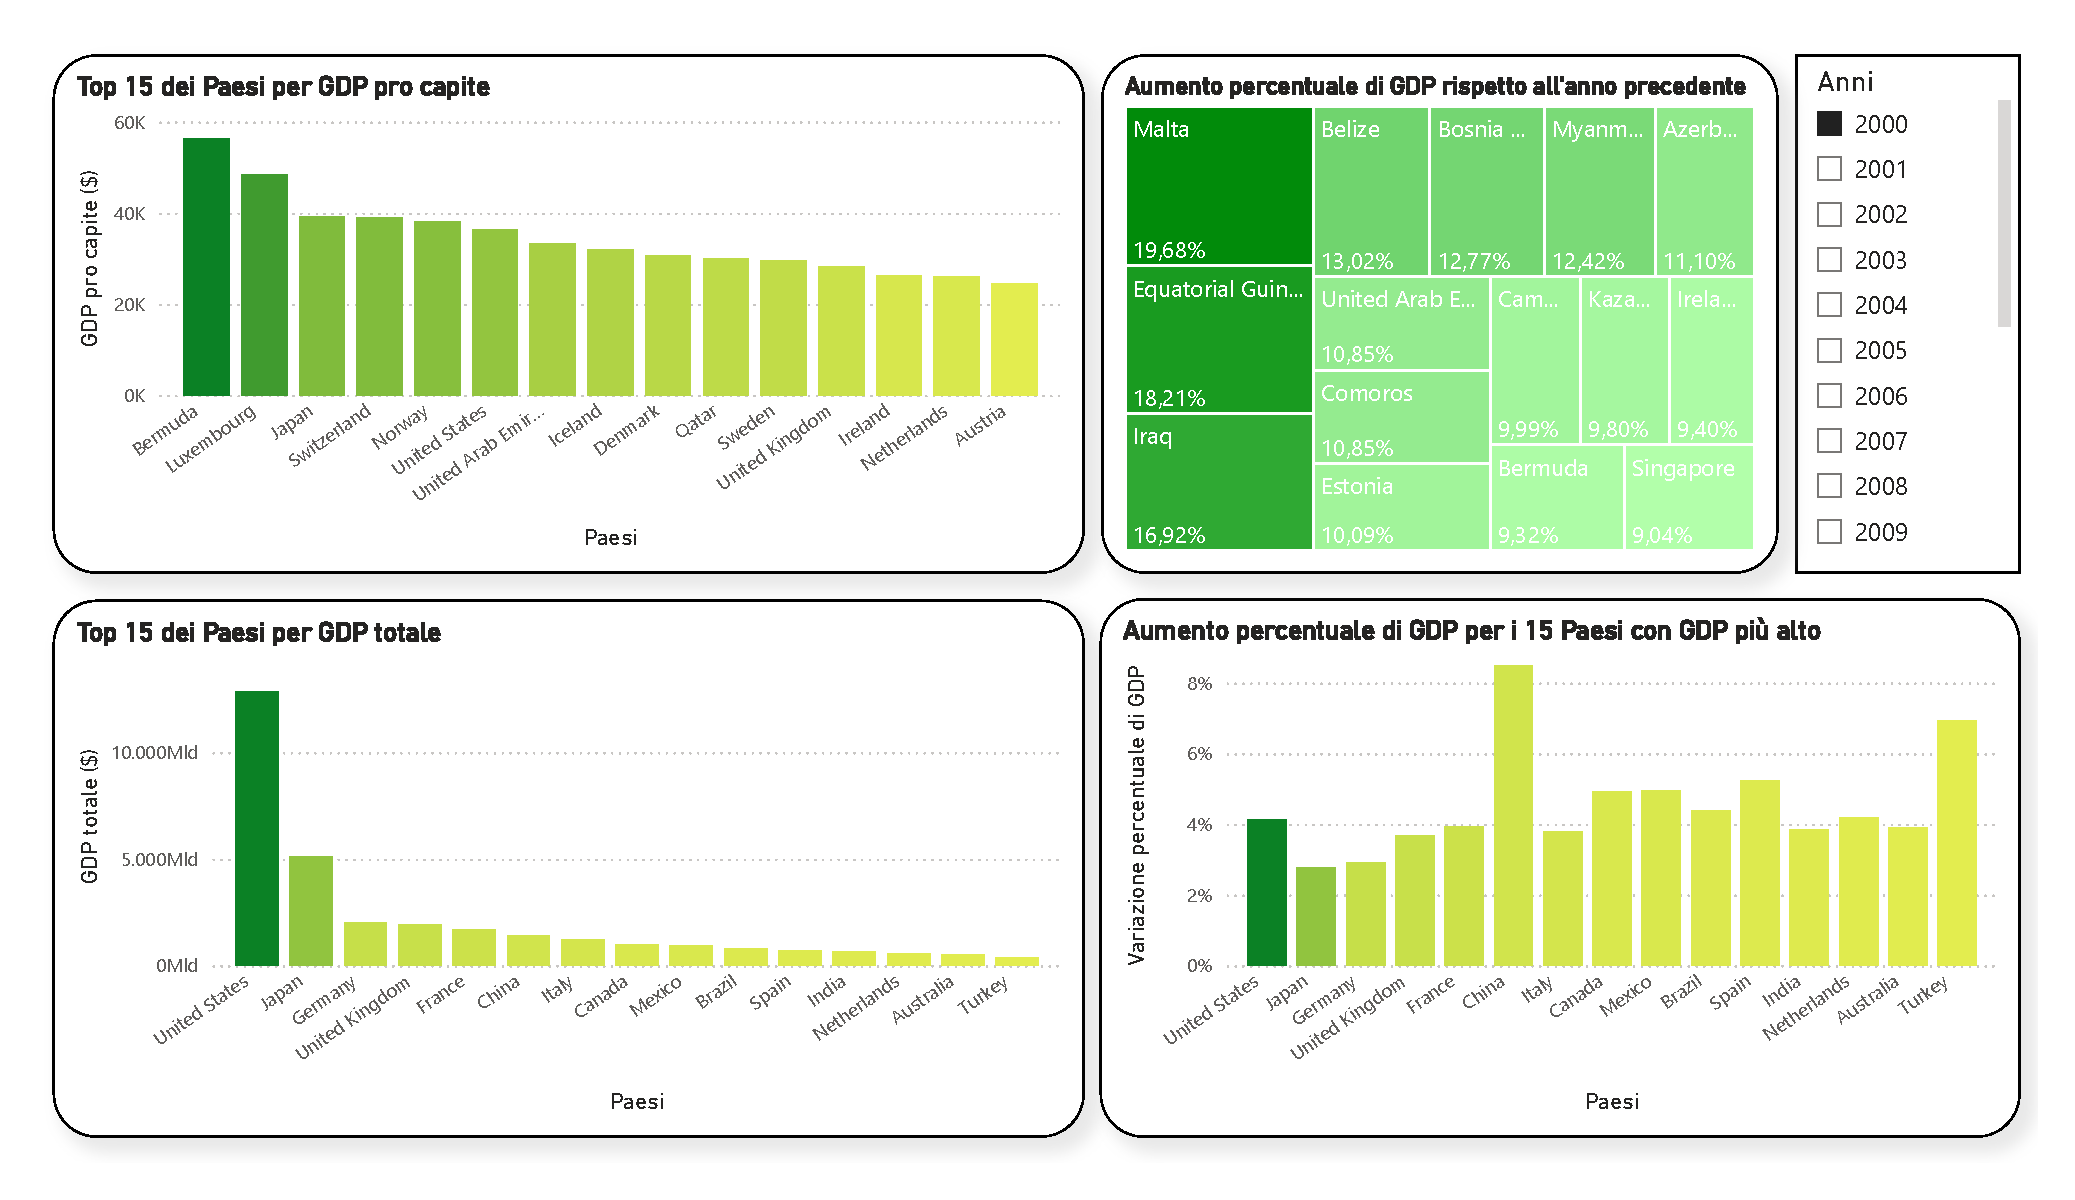
\includegraphics[width=0.98\linewidth]{capitolo_4/img4/PIL_Anno_2000.pdf}
    \caption{Analisi globale del GDP - Anno 2000}
    \label{fig:GDP_2000}
\end{figure}

\subsubsection{Struttura della Dashboard}
La seguente visualizzazione si articola in quattro grafici principali, ciascuno volto a rappresentare differenti aspetti dell’economia globale attraverso il prodotto interno lordo (GDP). Di seguito, una descrizione dettagliata di ciascun grafico:

\vspace{2mm} 
\begin{itemize} 
\item \textbf{Top 15 Paesi per GDP pro capite}: questo grafico a barre illustra i quindici Paesi con il più elevato prodotto interno lordo pro capite, espresso in dollari statunitensi (\$). Il GDP pro capite rappresenta un indicatore chiave per misurare la ricchezza media disponibile per ciascun cittadino all'interno di uno Stato, offrendo una prospettiva comparativa del benessere economico individuale su scala globale.
\item \textbf{Aumento percentuale del GDP rispetto all'anno precedente}: il grafico Treemap evidenzia la variazione percentuale del prodotto interno lordo di ciascun Paese rispetto all'anno precedente. Gli Stati sono ordinati in modo decrescente sulla base del tasso di crescita, consentendo un'immediata identificazione delle economie che hanno registrato le migliori performance in termini di espansione economica.
\item \textbf{Top 15 Paesi per GDP totale}: questo grafico a barre rappresenta i quindici Paesi con il GDP complessivo più elevato, espresso in dollari statunitensi (\$). Tale metrica riflette la dimensione assoluta dell'economia di ciascun Paese, offrendo un'indicazione del peso economico delle singole nazioni sullo scenario internazionale. Il GDP totale degli Stati è stato calcolato creando una colonna il cui valore è pari al prodotto tra \texttt{gdp\_per\_capita}, \texttt{Land\_Area} e \texttt{Density\_population}.
\item \textbf{Aumento percentuale del GDP per i 15 Paesi con GDP più alto}: in questo istogramma viene riportata la variazione percentuale annua del GDP dei quindici Paesi con il prodotto interno lordo totale più elevato. Il confronto consente di valutare non solo la dimensione economica assoluta, ma anche la dinamica evolutiva delle economie leader nel contesto globale.
\end{itemize}
\vspace{2mm}

Le analisi possono essere filtrate per uno specifico anno; in questo caso è stato selezionato l'anno 2000.

\subsubsection{Obiettivo dell'Analisi}
La Dashboard presentata offre una visione d'insieme chiara e strutturata della situazione economica dei principali Stati a livello globale. Attraverso una combinazione di indicatori, essa consente di analizzare in modo comparativo e dinamico le diverse dimensioni della ricchezza e dello sviluppo economico.

Uno degli elementi di maggiore rilevanza è il confronto tra il prodotto interno lordo pro capite e il prodotto interno lordo totale. Questa distinzione permette di adottare una doppia prospettiva: da un lato, si misura la capacità media di generazione di valore per singolo abitante, offrendo un indicatore diretto del benessere economico individuale; dall'altro, si valuta l'ampiezza e la forza complessiva dell'economia di ciascun Paese, elemento fondamentale per comprendere il peso economico relativo delle diverse nazioni sullo scenario mondiale. Tali dimensioni, pur strettamente correlate, non sempre coincidono, e il loro raffronto rappresenta uno strumento prezioso per analizzare non solo la distribuzione della ricchezza, ma anche le eventuali disparità tra le economie avanzate e quelle in via di sviluppo.

A completamento di questa analisi statica, la Dashboard include anche un'analisi dinamica tramite la variazione percentuale del GDP rispetto all'anno precedente. Questa metrica, applicata sia a livello globale che per le economie più avanzate, consente di osservare l'evoluzione della crescita economica, identificando tendenze espansive o segnali di rallentamento, utili per definire strategie di sviluppo, investimenti e valutare i rischi associati a specifiche aree geografiche.

Questa panoramica economica rappresenta inoltre un passaggio propedeutico per ulteriori approfondimenti in ambiti complementari, come ad esempio lo studio dell'impatto che la condizione economica degli Stati può avere sulle politiche ambientali. Comprendere il livello di sviluppo economico e la sua dinamica nel tempo è infatti essenziale per valutare la capacità e la disponibilità dei Paesi ad adottare misure efficaci per la sostenibilità e la transizione ecologica. Economie più solide e in crescita, in linea generale, dispongono di maggiori risorse da destinare a innovazione tecnologica, efficienza energetica e investimenti verdi; tuttavia, è necessario tenere conto anche di come tali risorse vengano effettivamente impiegate e delle priorità politiche dei singoli Stati.

In Figura \ref{GDP_3}, mostra la Dashboard filtrata per gli anni 2010 e 2019 (periodi analizzati anche nelle Dashboard precedenti). 
\begin{figure}[H]
    \centering
    \subfloat[\textbf{Anni 2010}]{%
        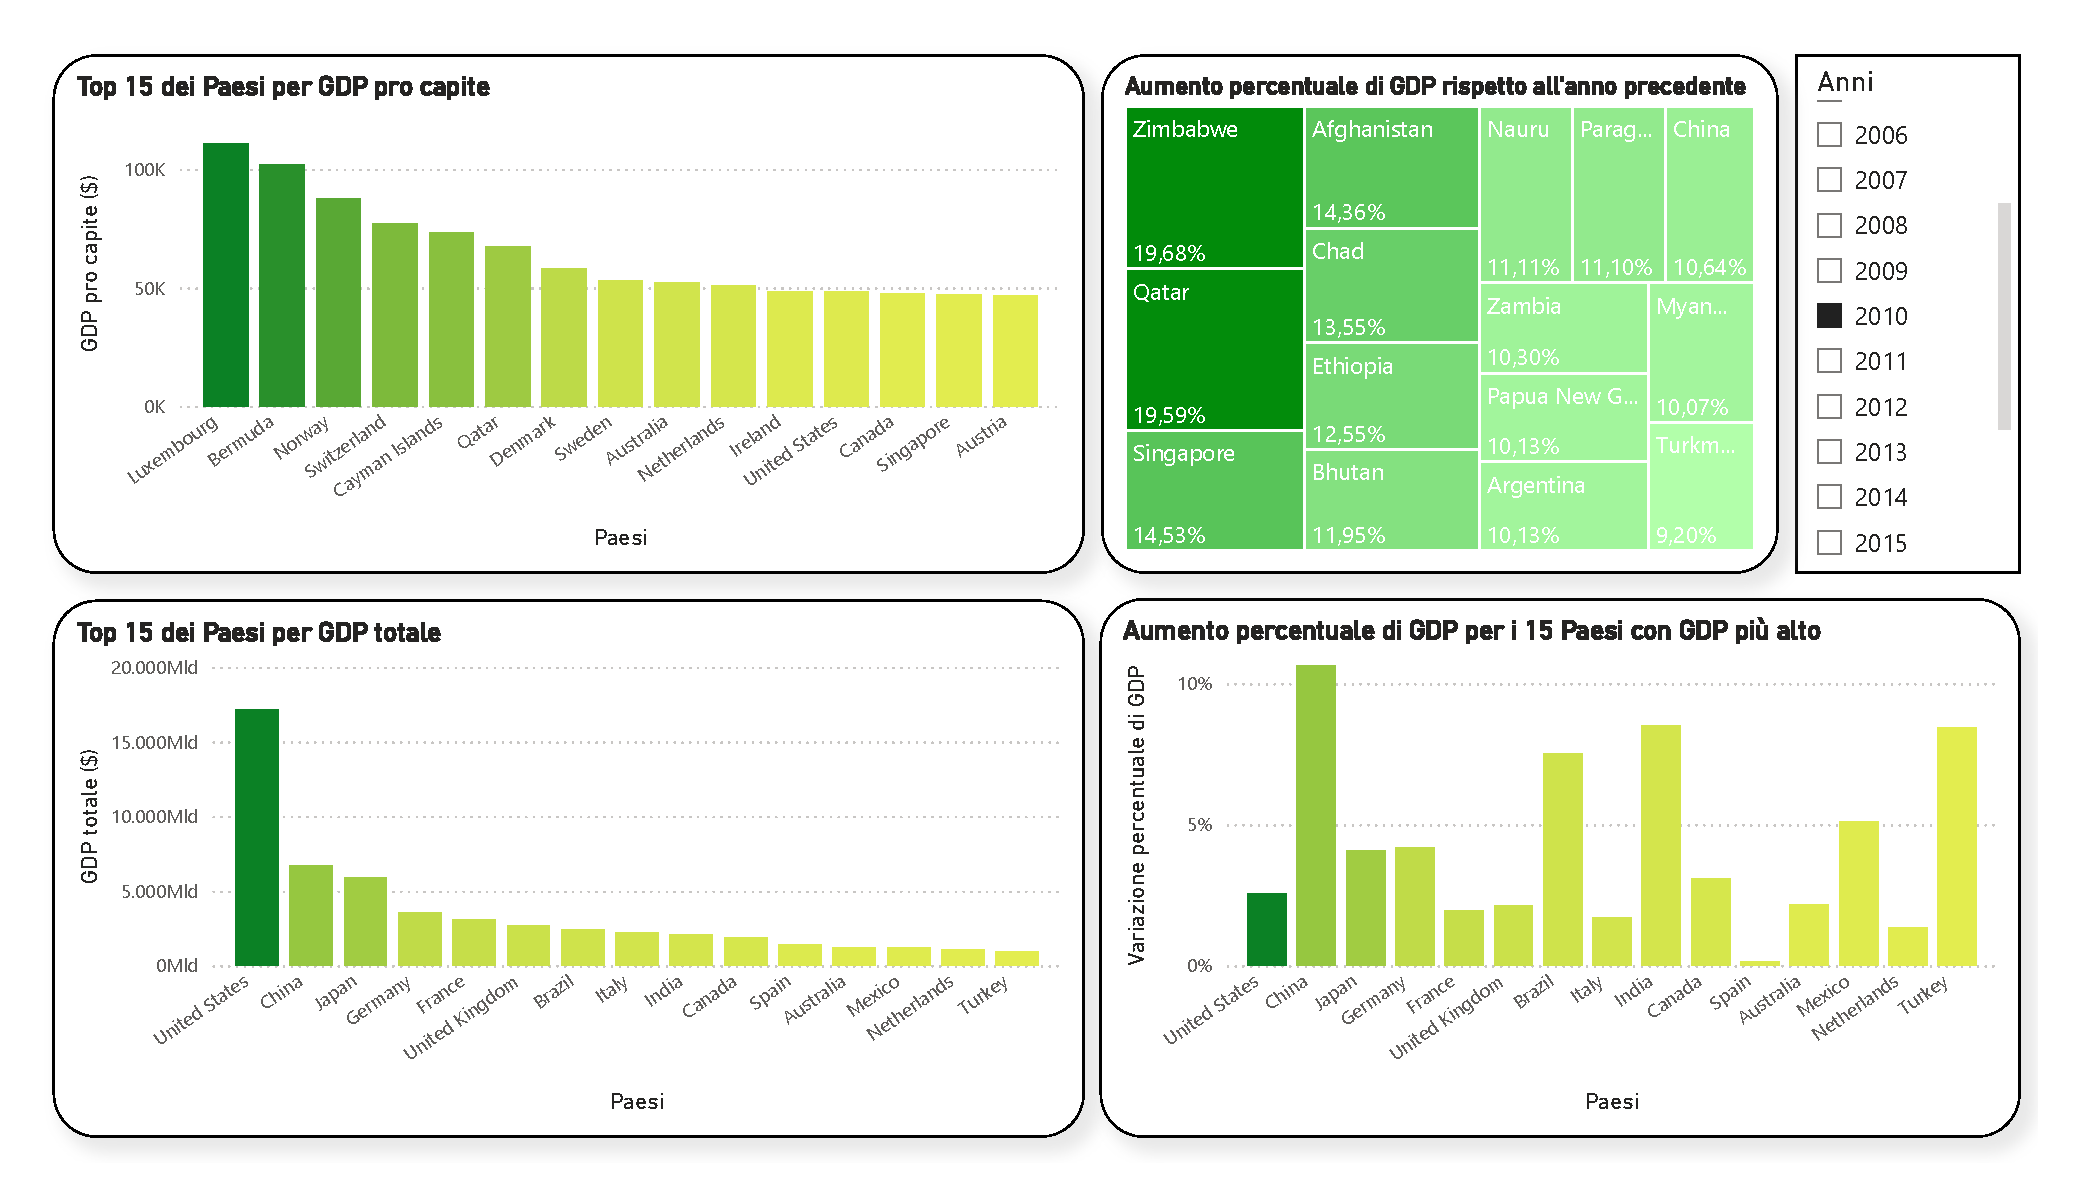
\includegraphics[width=0.9\textwidth]{capitolo_4/img4/PIL_Anno_2010.pdf}}\\
    \subfloat[\textbf{Anni 2019}]{%
        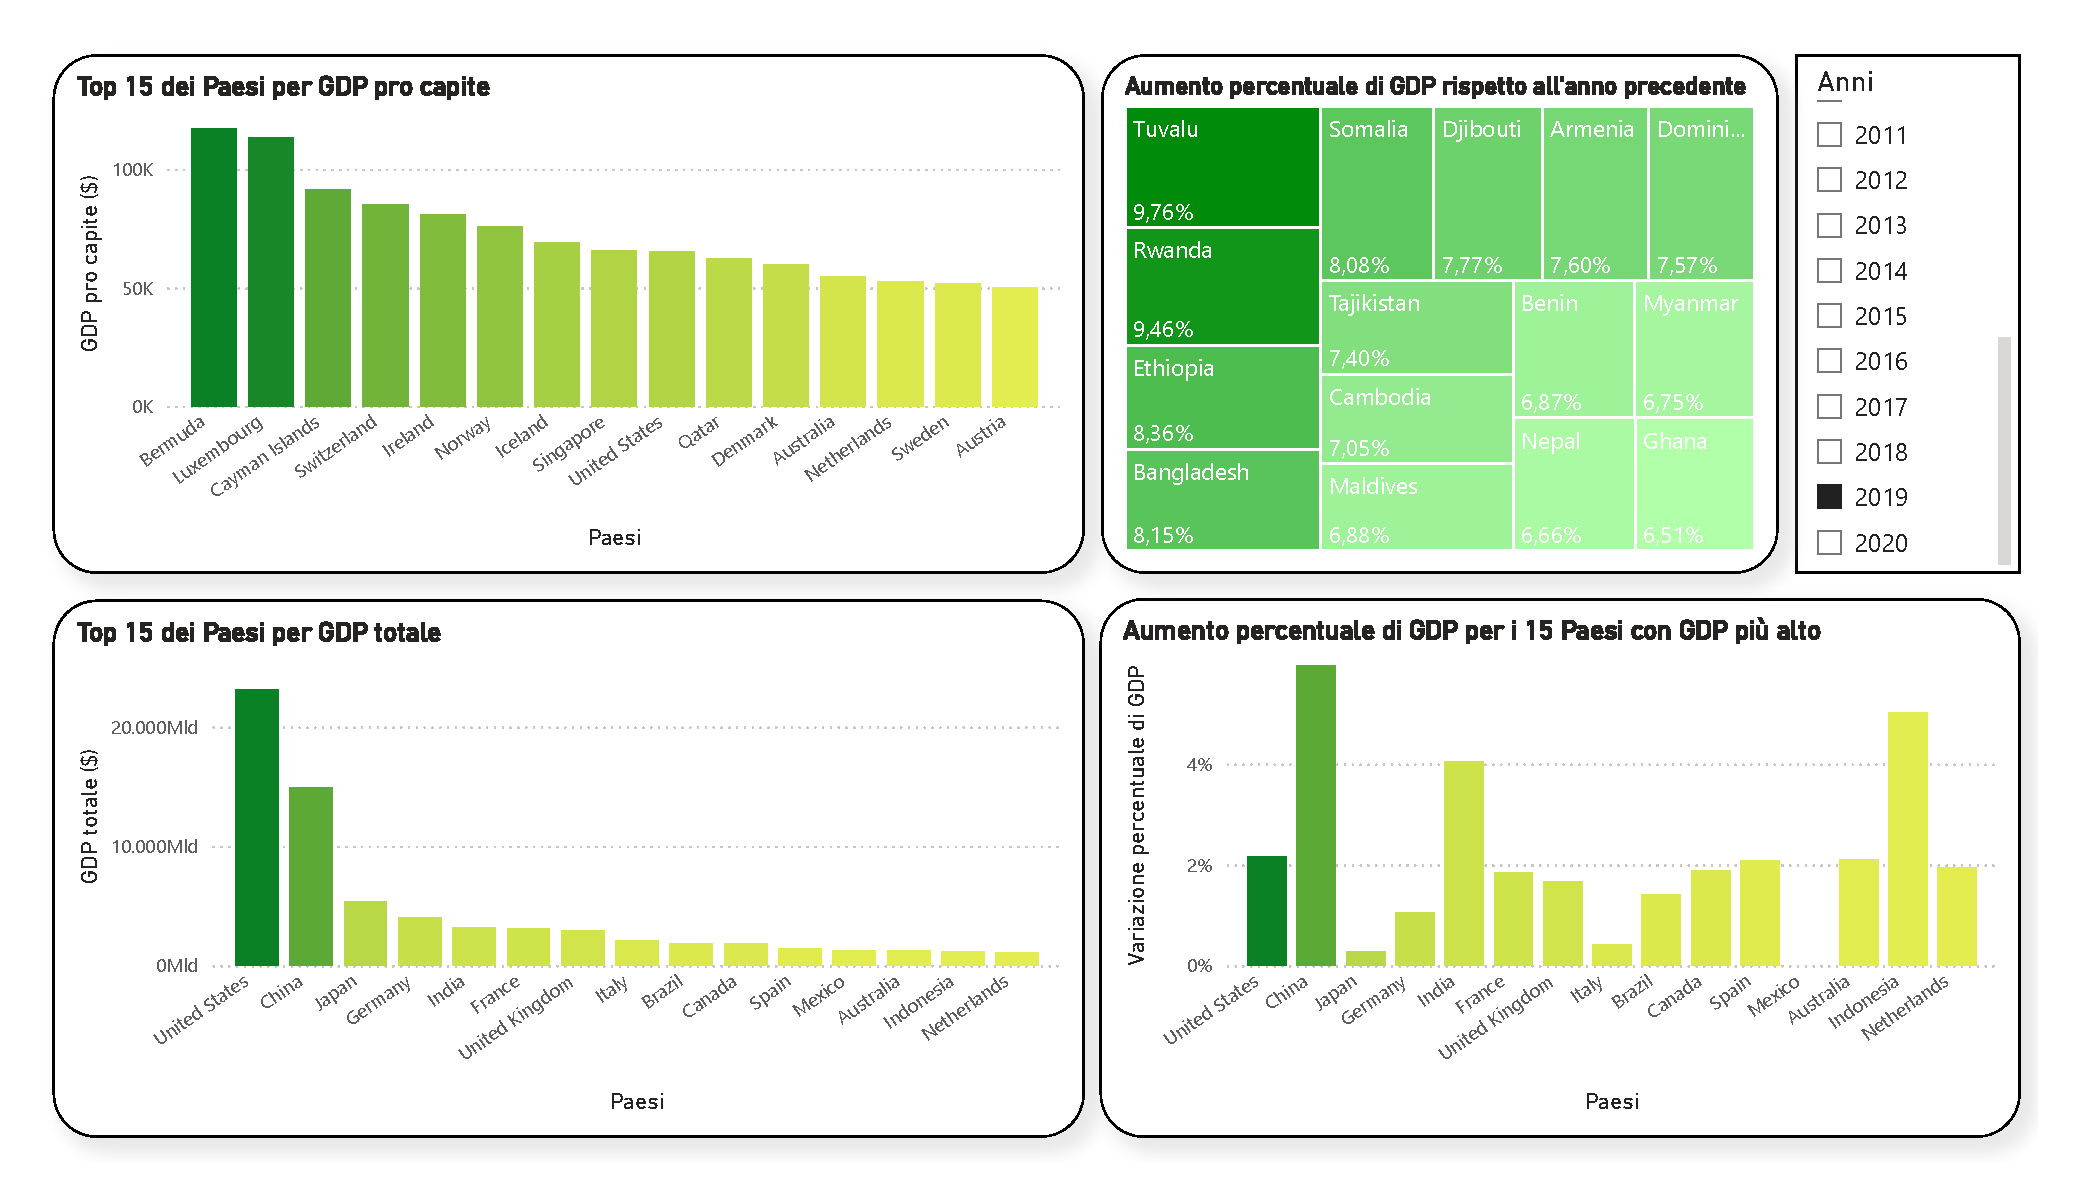
\includegraphics[width=0.9\textwidth]{capitolo_4/img4/PIL_Anno_2019.pdf}}
   \caption{Analisi globale del GDP - Anni 2010 e 2019}
  \label{GDP_3}
\end{figure}

\newpage
\subsection{Andamento delle emissioni di CO\textsubscript{2} in relazione alla crescita del GDP}
\label{GDP_1}

La Dashboard mostrata in Figura \ref{disp} sintetizza la relazione tra la media delle emissioni di CO\textsubscript{2} (espresso in kTon) e la media del GDP (espresso in dollari) dei dieci Paesi con il GDP più elevato. Questa visualizzazione consente di analizzare l'intensità carbonica delle principali economie mondiali, evidenziando il rapporto tra sviluppo economico e impatto ambientale.

\begin{figure}[h!]
    \centering
    \subfloat[\textbf{Risultati con USA e Cina}]{%
        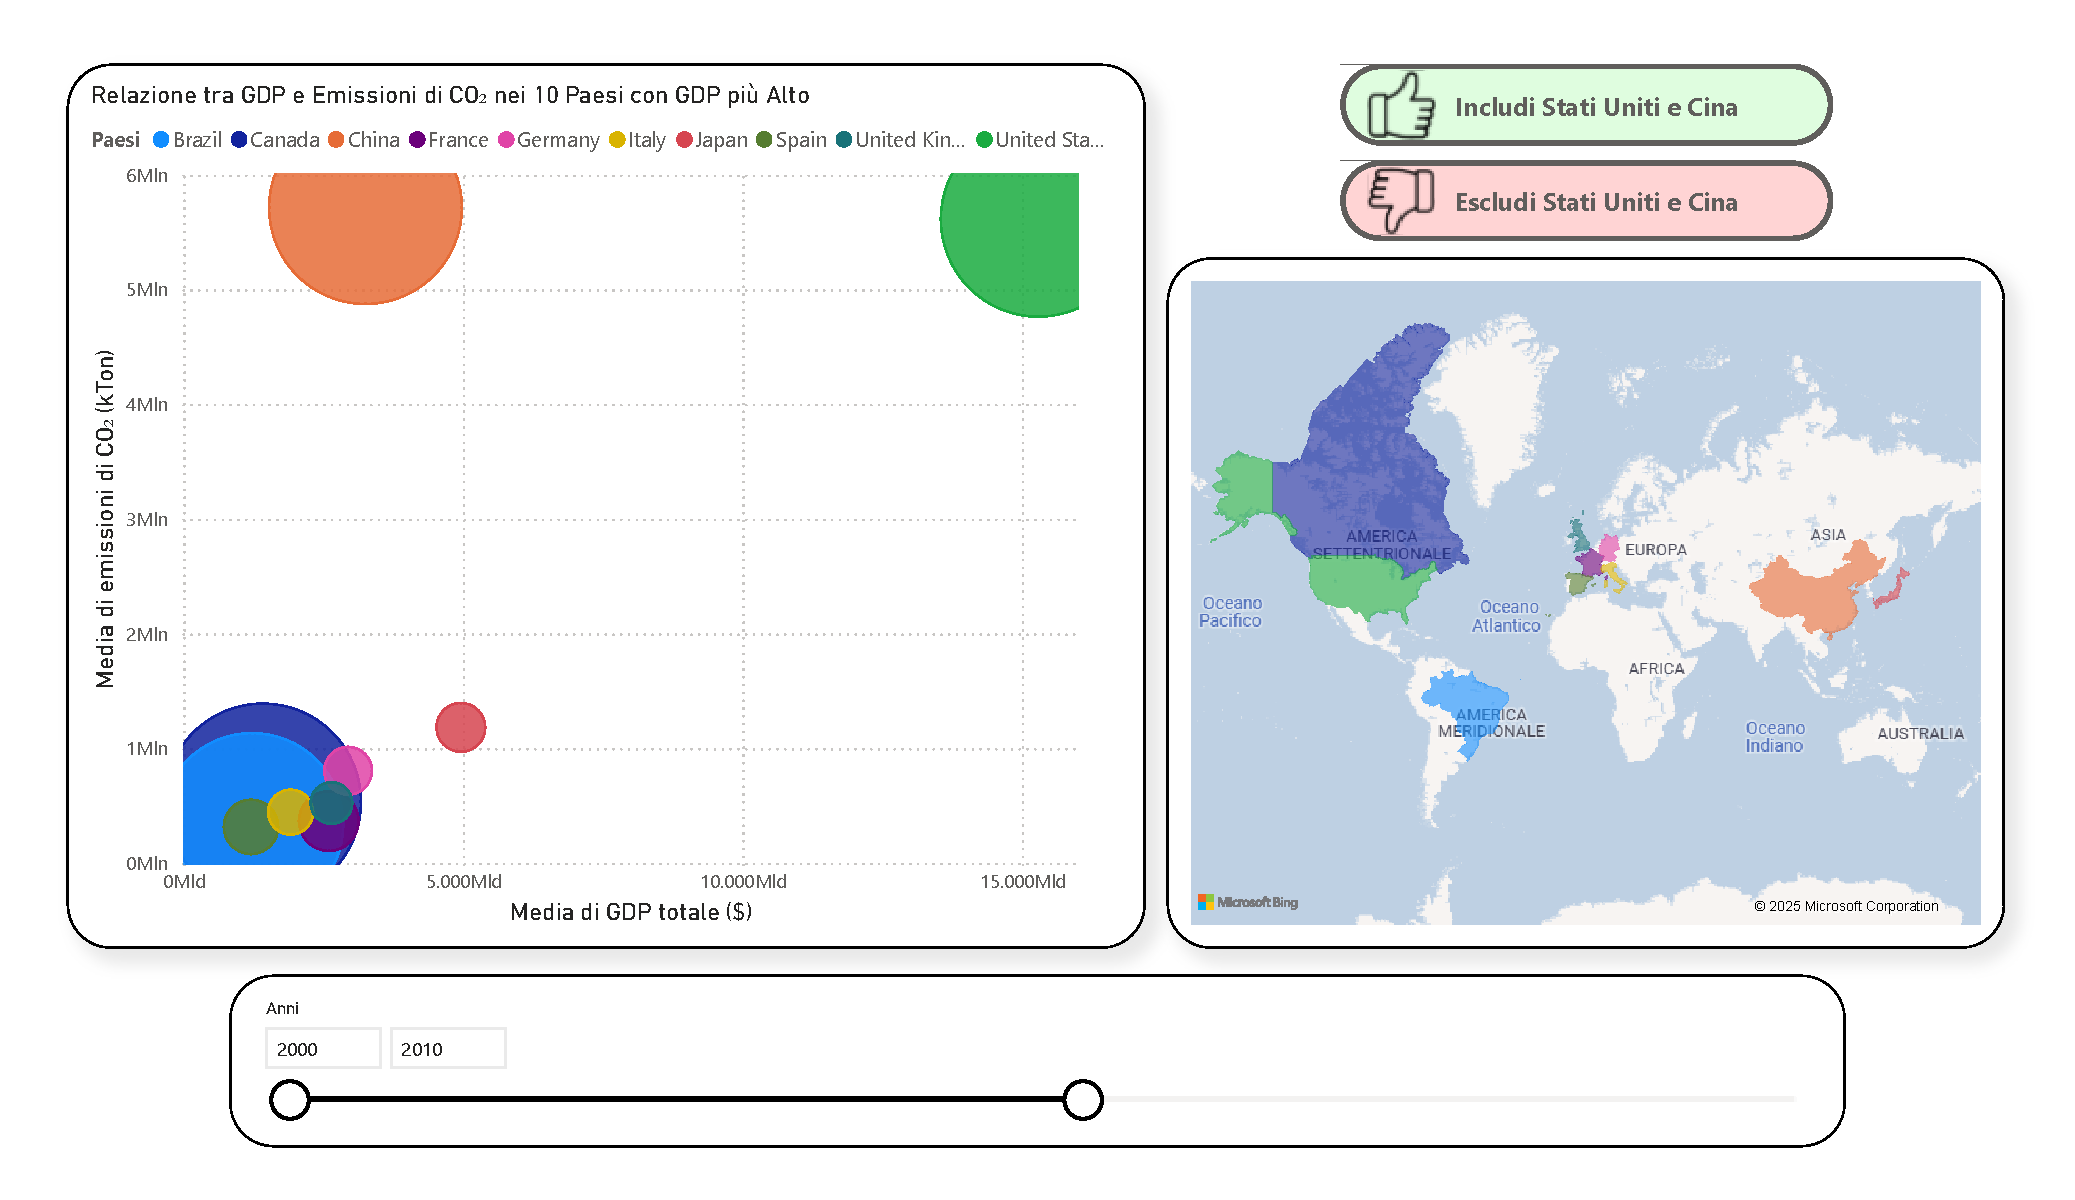
\includegraphics[width=0.9\textwidth]{capitolo_4/img4.1/CO2_GDP_2000_2010_conCinaeUSA.pdf}}\\
    \subfloat[\textbf{Risultati senza USA e Cina}]{%
        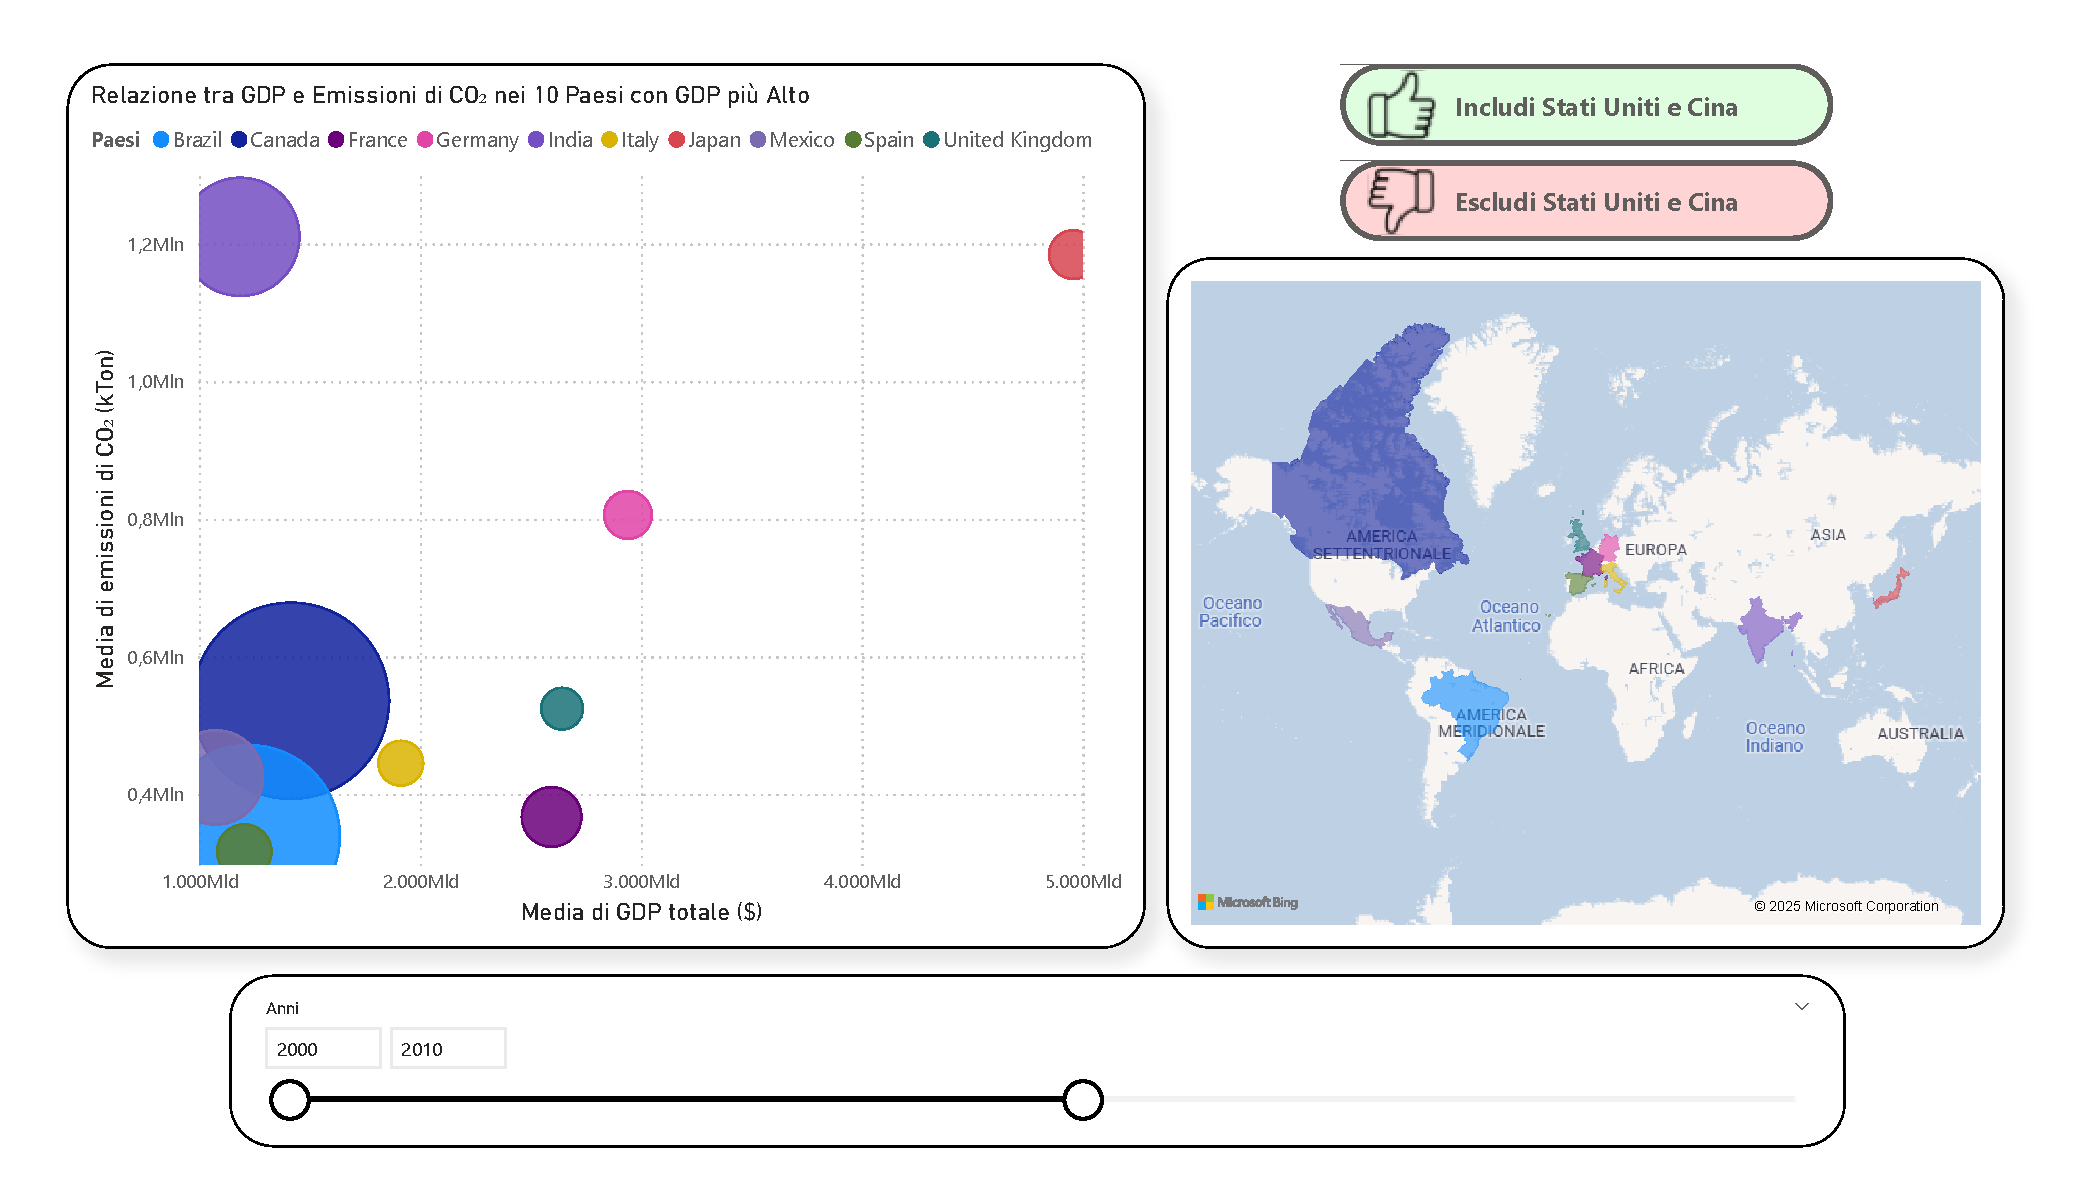
\includegraphics[width=0.9\textwidth]{capitolo_4/img4.1/CO2_GDP_2000_2010_senzaCinaeUSA.pdf}}
   \caption{Andamento delle emissioni di CO\textsubscript{2} in relazione alla crescita del GDP - Anni 2000-2010}
  \label{disp}
\end{figure}


\subsubsection{Struttura della Dashboard}
La Dashboard si compone di diversi elementi, progettati per favorire un'analisi dettagliata dei dati. Nella parte sinistra dell'interfaccia è presente un \textbf{Grafico a Dispersione}, il quale rappresenta visivamente la relazione tra due variabili chiave: la media del GDP, riportata sull'asse delle ascisse, e la media delle emissioni di CO\textsubscript{2}, visualizzata sull'asse delle ordinate. Ogni punto colorato nel grafico corrisponde a un singolo Stato e consente di confrontare, in modo intuitivo, l'intensità delle emissioni rispetto al livello medio di sviluppo economico.
La dimensione delle bolle è proporzionale all'area geografica dello Stato, mettendo in relazione l'estensione territoriale con il livello di emissioni. 

A supporto dell'analisi proposta nel grafico a dispersione, la Dashboard è arricchita da una serie di filtri interattivi e visualizzazioni supplementari, pensati per agevolare l'interpretazione dei risultati. In particolare, sono disponibili i seguenti strumenti:

\vspace{2mm} 
\begin{itemize}
\item \textit{Filtro temporale}, che consente di selezionare l'intervallo di anni oggetto di analisi, compreso tra il 2000 e il 2019; 
\item \textit{Pulsanti} creati utilizzando i segnalibri di Power BI per consentire la selezione o la deselezione della visualizzazione dei dati relativi a Cina e Stati Uniti;
\begin{myoutline}
    \textbf{Nota}:l'inserimento dei pulsanti per la selezione di Stati Uniti e Cina è motivato dalla necessità di bilanciare la visualizzazione dei dati: i risulati relativi a questi due Paesi tendono a sovrastare l'analisi complessiva, rendendo meno visibili le dinamiche degli altri Stati. La possibilità di escluderli temporaneamente consente una lettura più chiara e approfondita dei dati relativi agli altri Paesi, migliorando la comprensione delle tendenze globali.
\end{myoutline}
\item \textit{Visualizzazione geografica interattiva}, che mostra la distribuzione degli Stati a livello mondiale, ciascuno rappresentato con una colorazione coerente con quella utilizzata nel grafico a dispersione. 
\end{itemize}
\vspace{2mm}

\subsubsection{Obiettivo dell'Analisi}
La presente Dashboard è stata progettata con l'obiettivo di fornire un'analisi approfondita della relazione tra lo sviluppo economico e l'impatto ambientale a livello globale, utilizzando come principali indicatori il GDP e le emissioni medie annue di anidride carbonica. Questo strumento consente di osservare, in modo congiunto, l'andamento di questi due parametri per i diversi Paesi, al fine di identificare eventuali correlazioni o discrepanze tra la crescita economica e l'inquinamento atmosferico.

\begin{figure}[h!]
    \centering
    \subfloat[\textbf{Risultati con USA e Cina}]{%
        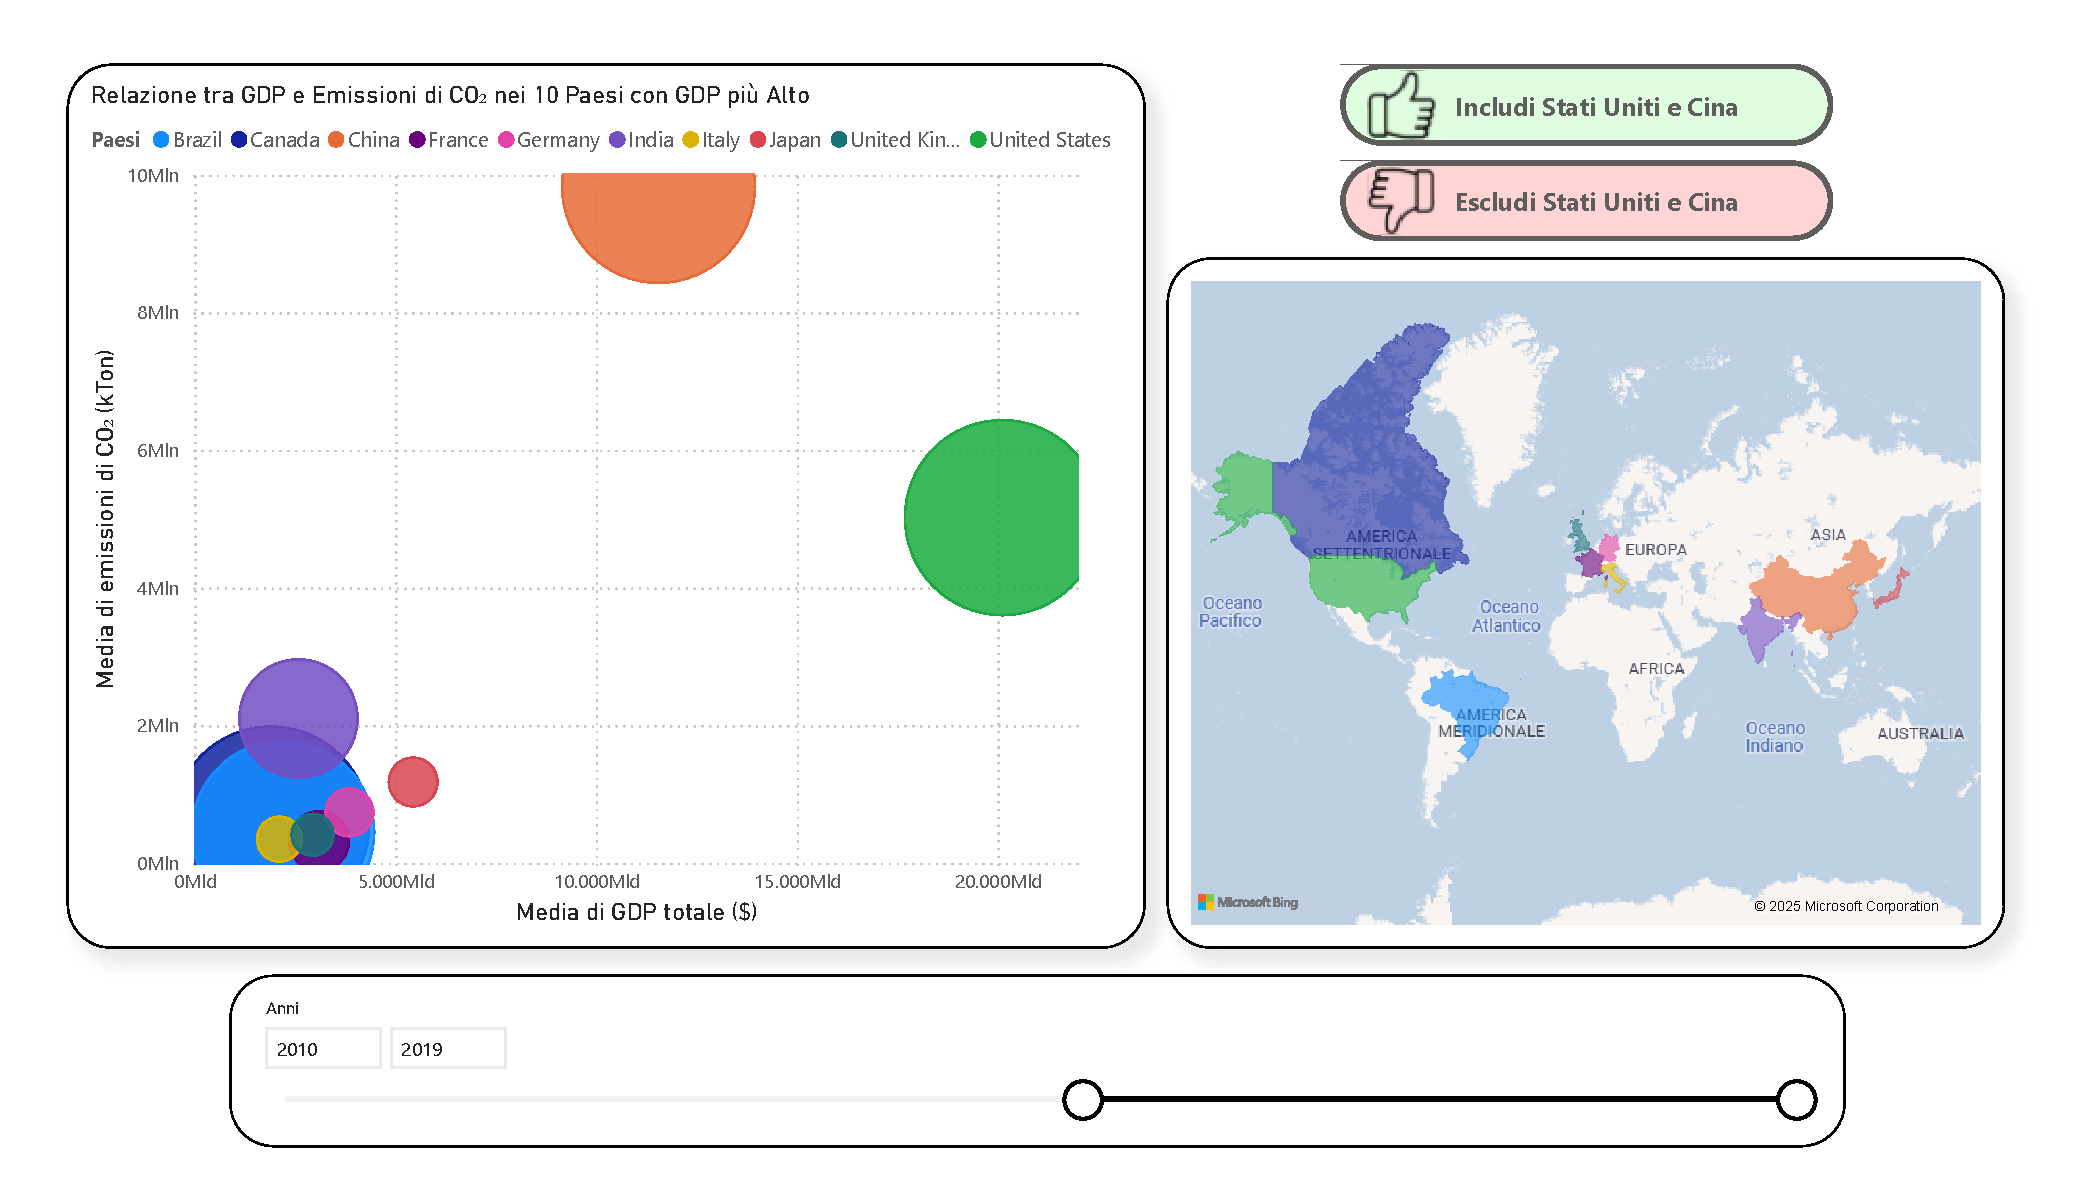
\includegraphics[width=0.9\textwidth]{capitolo_4/img4.1/CO2_GDP_2010_2019_conCinaeUSA.pdf}}\\
    \subfloat[\textbf{Risultati senza USA e Cina}]{%
        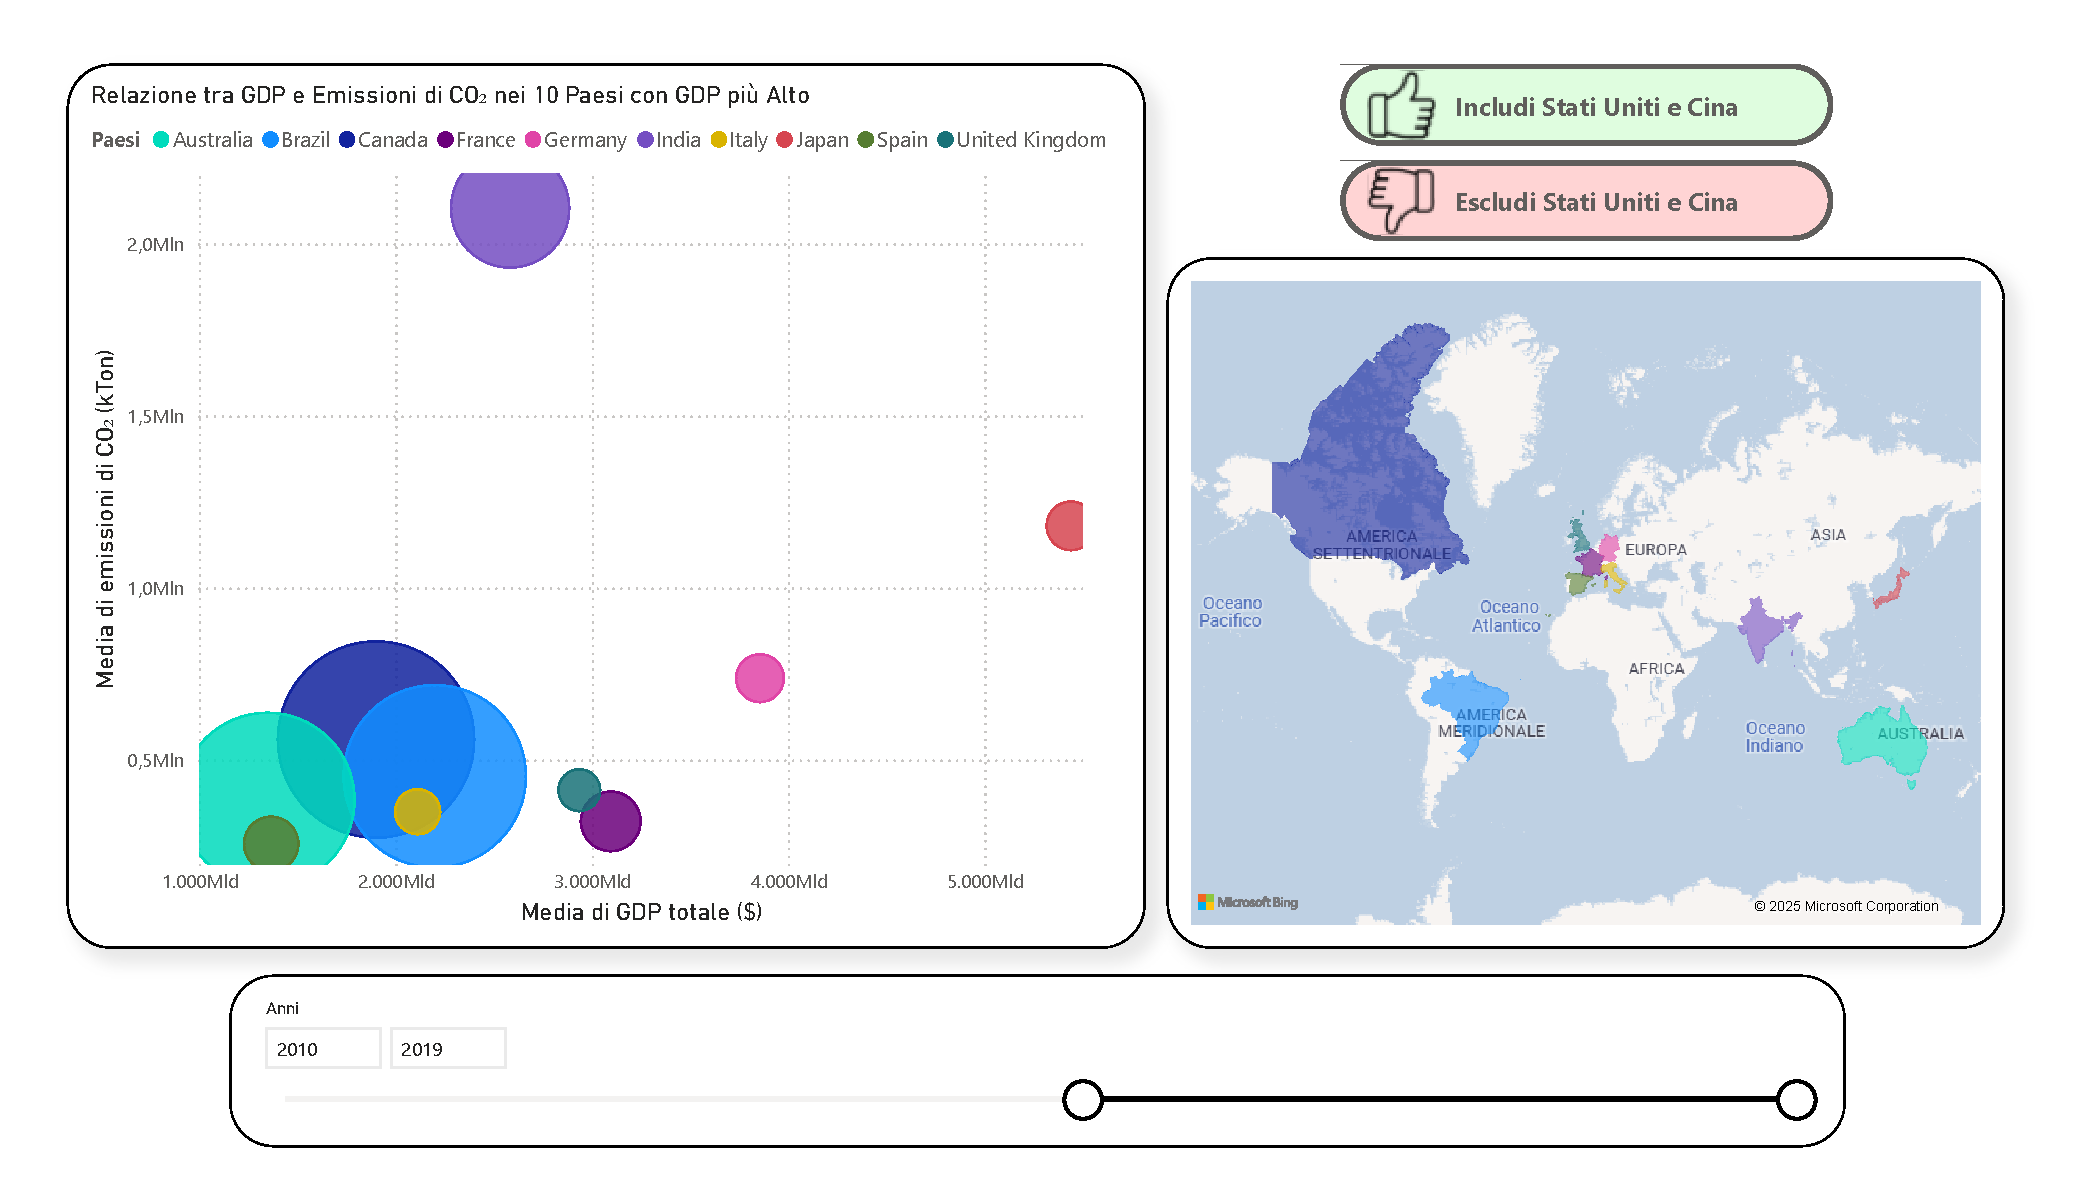
\includegraphics[width=0.9\textwidth]{capitolo_4/img4.1/CO2_GDP_2010_2019_senzaCinaeUSA.pdf}}
   \caption{Andamento delle emissioni di CO\textsubscript{2} in relazione alla crescita del GDP - Anni 2010-2019}
  \label{disp_1}
\end{figure}

Osservando la Figura \ref{disp} e la Figura \ref{disp_1}, è evidente che non esiste una correlazione diretta e lineare tra la ricchezza economica di un Paese e le sue emissioni di CO\textsubscript{2}. Ad esempio, come si può notare nella Figura \ref{disp_1}, Paesi come il Giappone (rappresentato dal \textcolor[RGB]{220,97,106}{colore}) presentano un GDP estremamente elevato, ma emissioni di CO\textsubscript{2} relativamente contenute, rispetto all'India (rappresentata dal \textcolor[RGB]{137, 104, 203}{colore}), la quale, pur avendo un GDP inferiore, mostra un livello di emissioni significativamente più elevato. Questo fenomeno non può essere spiegato nemmeno in relazione alla superficie territoriale dei Paesi: ad esempio, l'Australia (rappresentata dal \textcolor[RGB]{38, 224, 198}{colore}), nonostante un'area geografica molto ampia, presenta emissioni di CO\textsubscript{2} relativamente contenute.

Questa discrepanza suggerisce che la relazione tra sviluppo economico e inquinamento non può essere valutata solo attraverso il GDP, ma deve considerare anche altri fattori, tra cui l'efficienza energetica, l'adozione di tecnologie verdi e le politiche di sostenibilità adottate dai singoli Paesi. 

\newpage
\subsection{Andamento produzione di energia rinnovabile rispetto alla crescita del GDP}
La Dashboard, presentata nella Figura \ref{disp_rinn}, fornisce una rappresentazione visiva sintetica della relazione tra la produzione media di energia rinnovabile (espressa in TWh) e la media di GDP dei dieci Paesi con il GDP più elevato. Questa visualizzazione consente di esaminare in modo dettagliato la generazione di energia rinnovabile nelle principali economie mondiali, evidenziando le connessioni tra lo sviluppo economico e le politiche energetiche adottate dai diversi Stati.

\begin{figure}[h!]
    \centering
    \subfloat[\textbf{Risultati con USA e Cina}]{%
        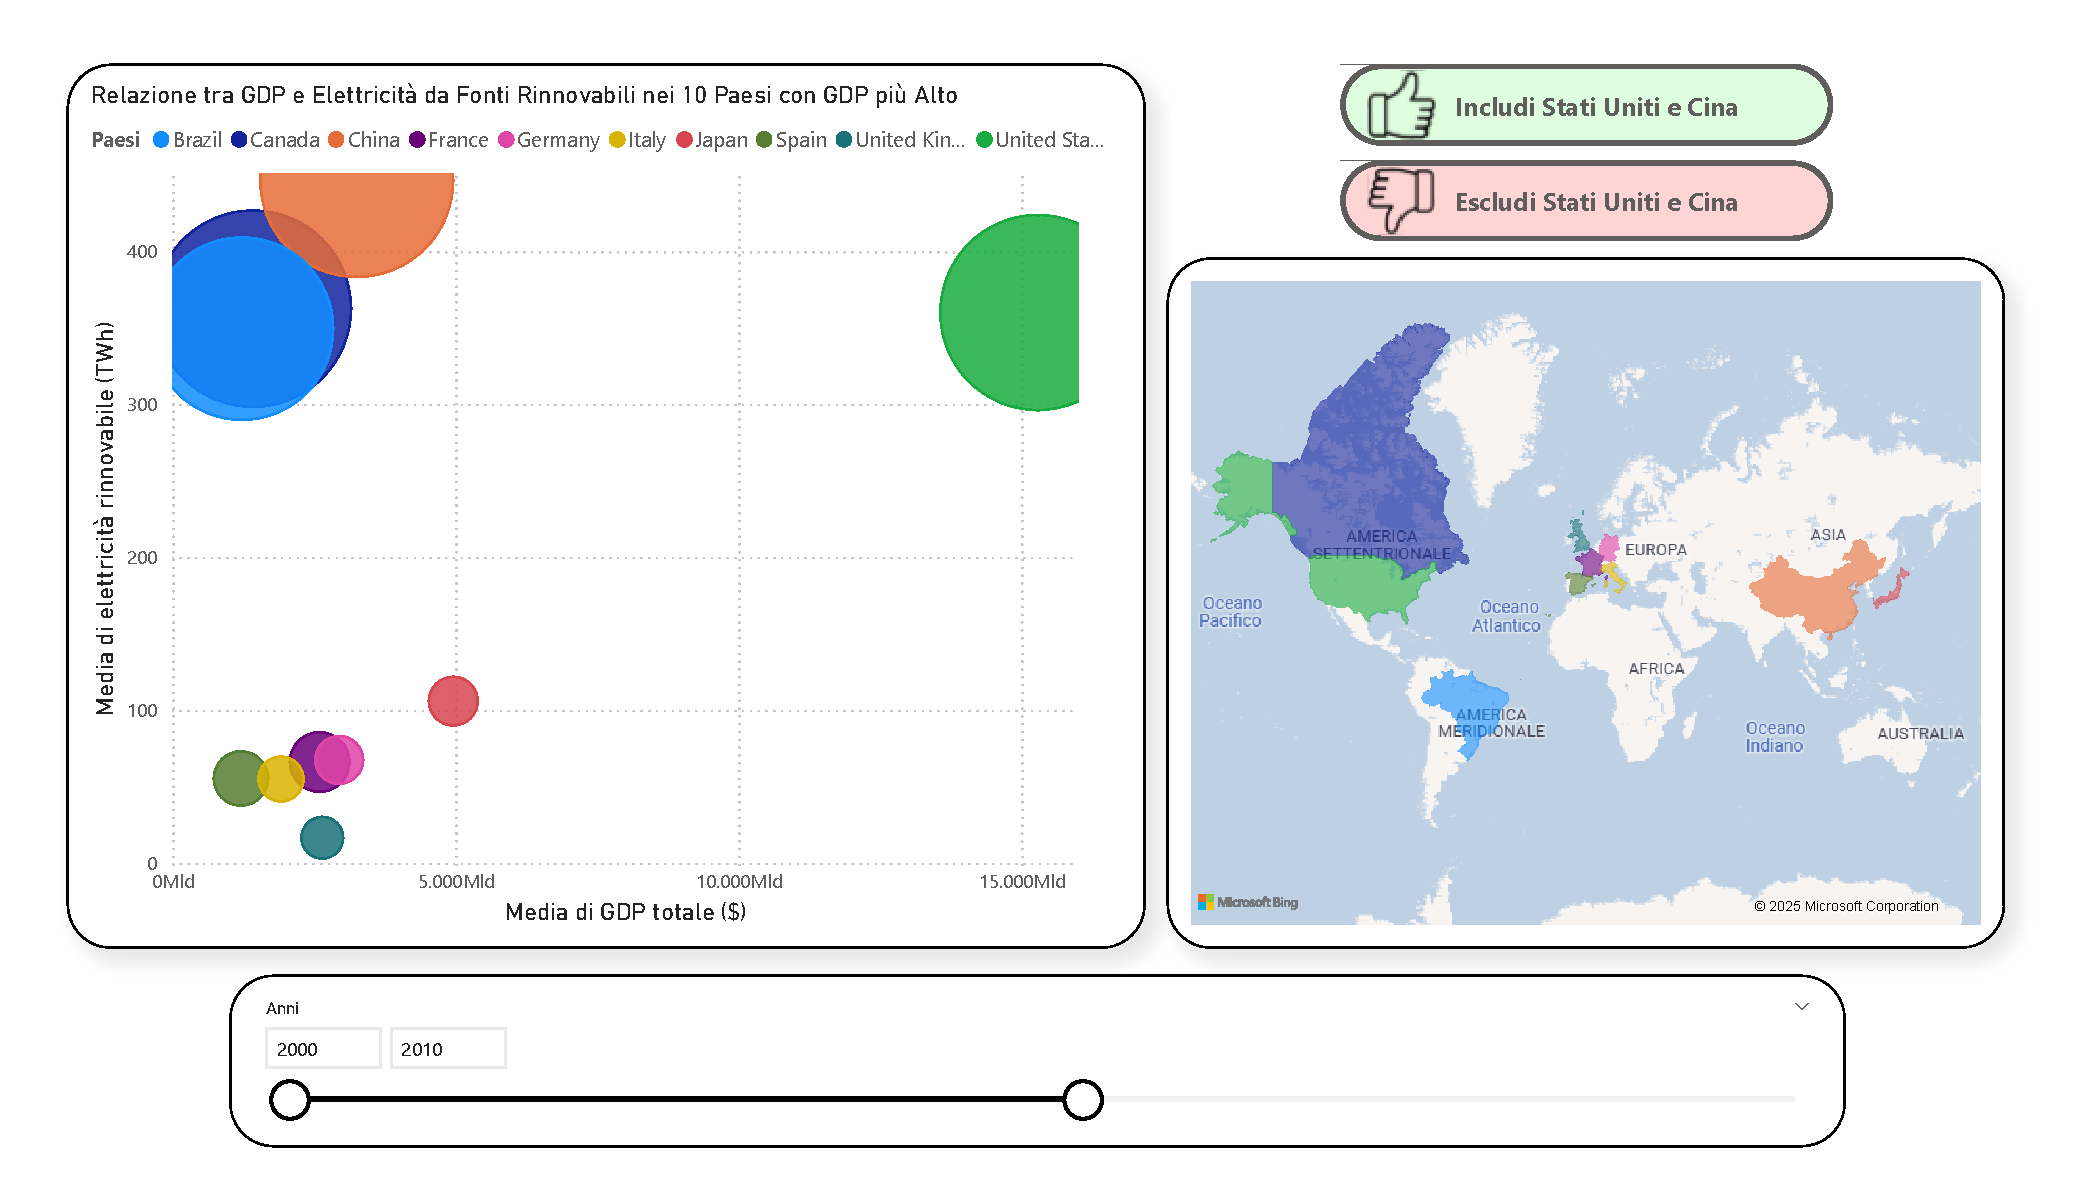
\includegraphics[width=0.9\textwidth]{capitolo_4/img4.1/Rinnovabile_GDP_2000_2010_conCinaeUSA.pdf}}\\
    \subfloat[\textbf{Risultati senza USA e Cina}]{%
        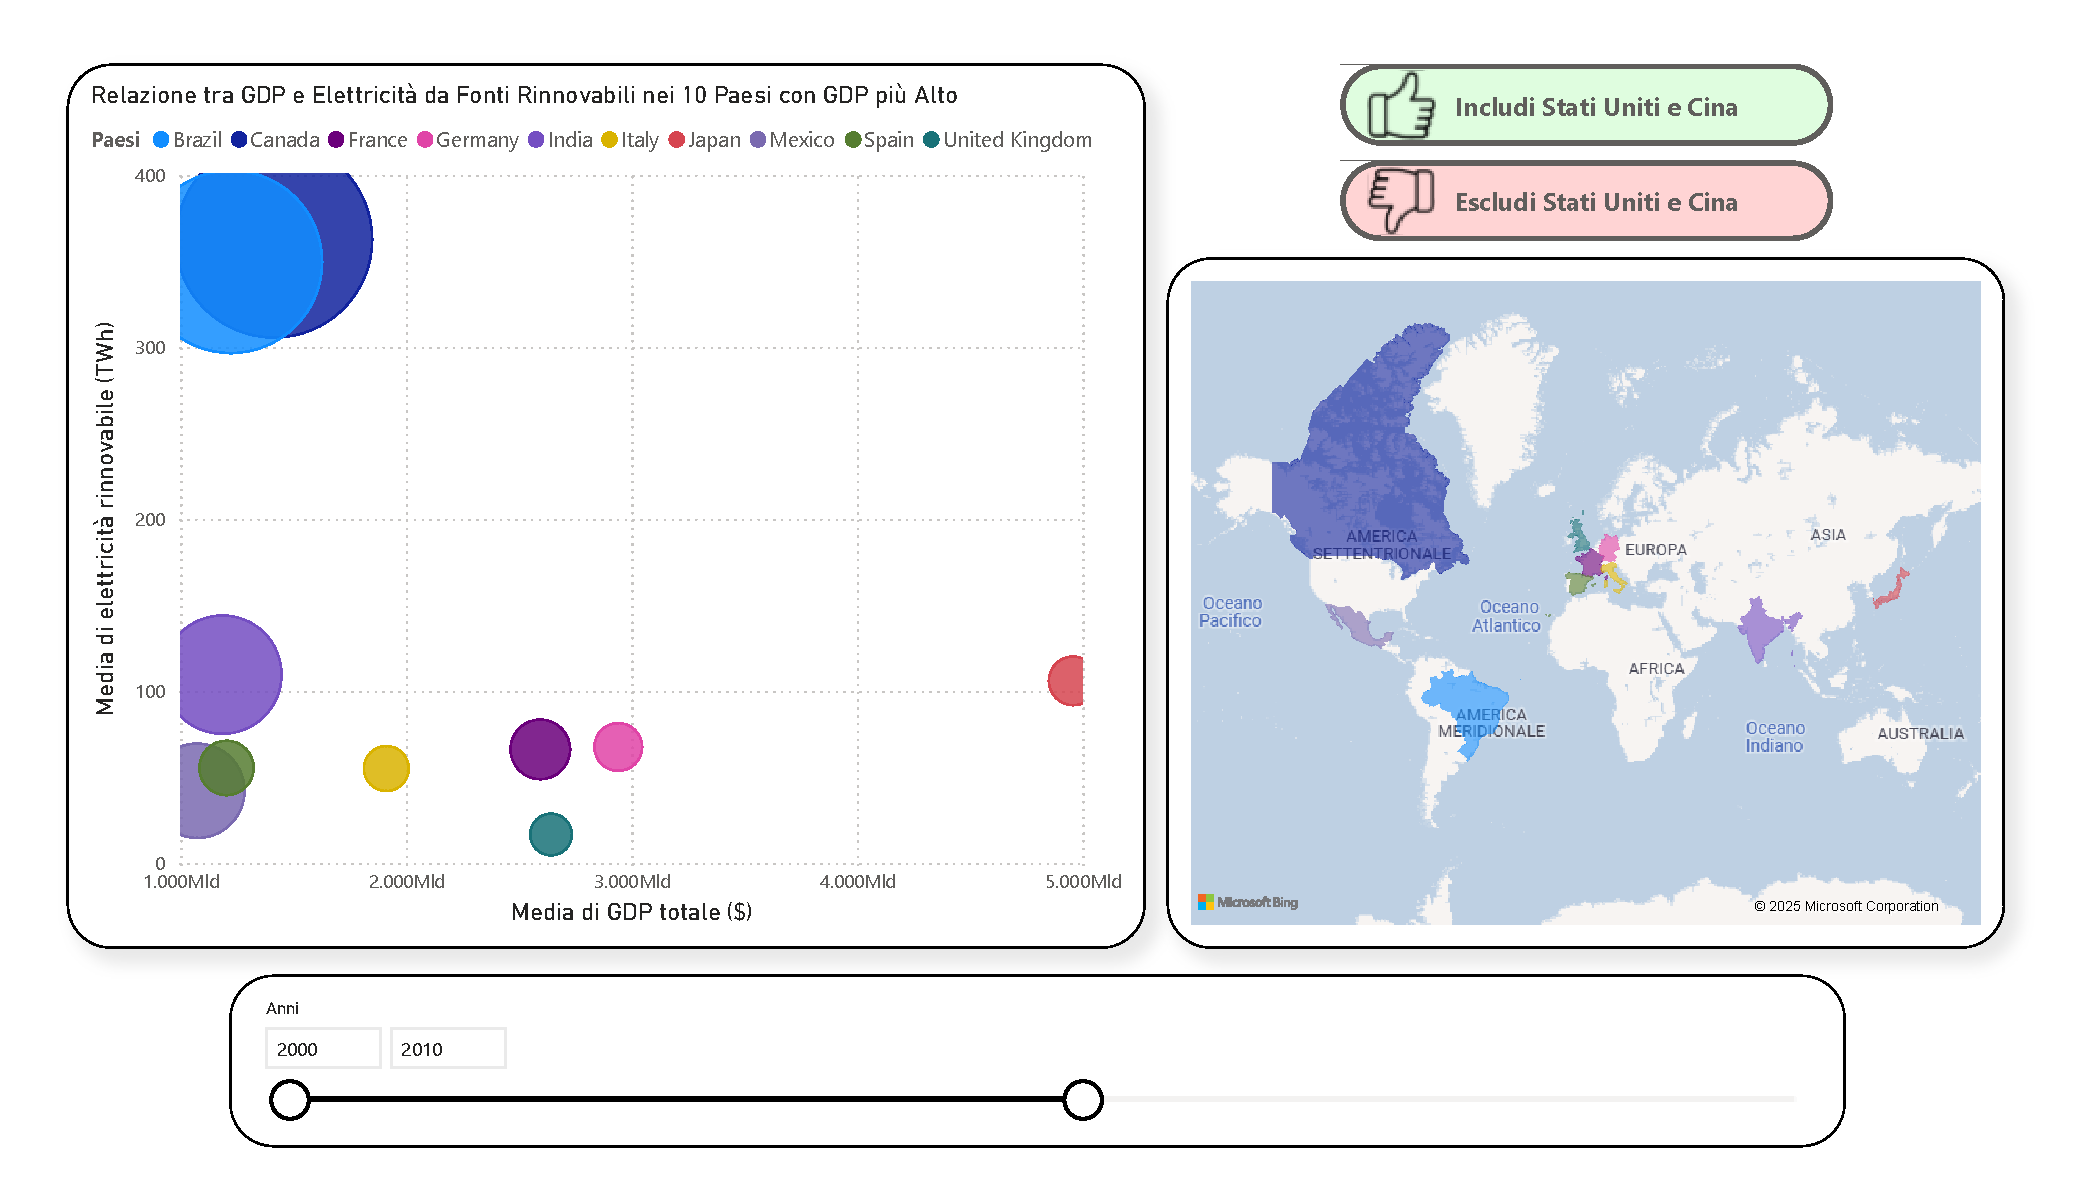
\includegraphics[width=0.9\textwidth]{capitolo_4/img4.1/Rinnovabile_GDP_2000_2010_senzaCinaeUSA.pdf}}
   \caption{Andamento della produzione di energia rinnovabile rispetto alla crescita del GDP - Anni 2000-2010}
  \label{disp_rinn}
\end{figure}

\subsubsection{Struttura della Dashboard}
La Dashboard è progettata per facilitare un'analisi dettagliata e completa dei dati. Nella parte sinistra dell'interfaccia, si trova un grafico a dispersione, creato per visualizzare la relazione tra due variabili chiave: la media del GDP (espressa in dollari), rappresentata sull'asse delle ascisse, e la produzione media di elettricità rinnovabile, riportata sull'asse delle ordinate.

Ogni punto colorato nel grafico corrisponde a un singolo Paese e consente di confrontare, in modo visivo e intuitivo, il livello di produzione di elettricità rinnovabile con il relativo livello di sviluppo economico, evidenziando tendenze e possibili anomalie. La dimensione delle bolle è proporzionale all'area geografica del Paese, correlando l'estensione territoriale con la quantità di elettricità rinnovabile prodotta.

Questa visualizzazione consente di osservare non solo la distribuzione globale dei Paesi in termini di produzione di energia rinnovabile, ma anche come le economie più grandi si confrontano con quelle più piccole, sia in termini di produzione energetica che di sviluppo economico.

Analogamente a quanto descritto nella Sezione \ref{GDP_1}, la Dashboard include una serie di filtri interattivi progettati per affinare l'analisi e personalizzare la visualizzazione dei dati in base alle esigenze dell'utente:

\vspace{2mm} 
\begin{itemize} 
\item \textit{Filtro temporale}: permette di definire l'intervallo cronologico da analizzare, selezionabile tra gli anni 2000 e 2019; 
\item \textit{Pulsanti}: consentono la selezione o la deselezione della visualizzazione dei dati relativi a Stati Uniti e Cina; 
\item \textit{Visualizzazione geografica}: propone una mappa interattiva in cui i Paesi sono evidenziati con una colorazione coerente con quella adottata nel grafico a dispersione. 
\end{itemize} 
\vspace{2mm}

\subsubsection{Obiettivo dell'Analisi}
La Dashboard presentata è stata sviluppata con l'intento di offrire un'analisi dettagliata della relazione tra sviluppo economico e produzione di energia rinnovabile a livello globale, facendo uso di due indicatori chiave: il GDP e la quantità media di energia rinnovabile generata. Attraverso un'integrazione visiva di questi parametri, lo strumento permette di esplorare l'evoluzione economica dei Paesi e il loro impegno nella transizione energetica, facilitando l'individuazione di possibili correlazioni, divergenze o tendenze significative.

La Figura \ref{disp_rinn} e la Figura \ref{disp_2_rinn} offrono un'analisi dettagliata dei primi dieci Paesi per PIL nei periodi 2000-2010 e 2010-2019, con l'obiettivo di fornire una panoramica rappresentativa dello scenario globale in termini di produzione di energia da fonti rinnovabili.

\begin{figure}[h!]
    \centering
    \subfloat[\textbf{Risultati con USA e Cina}]{%
        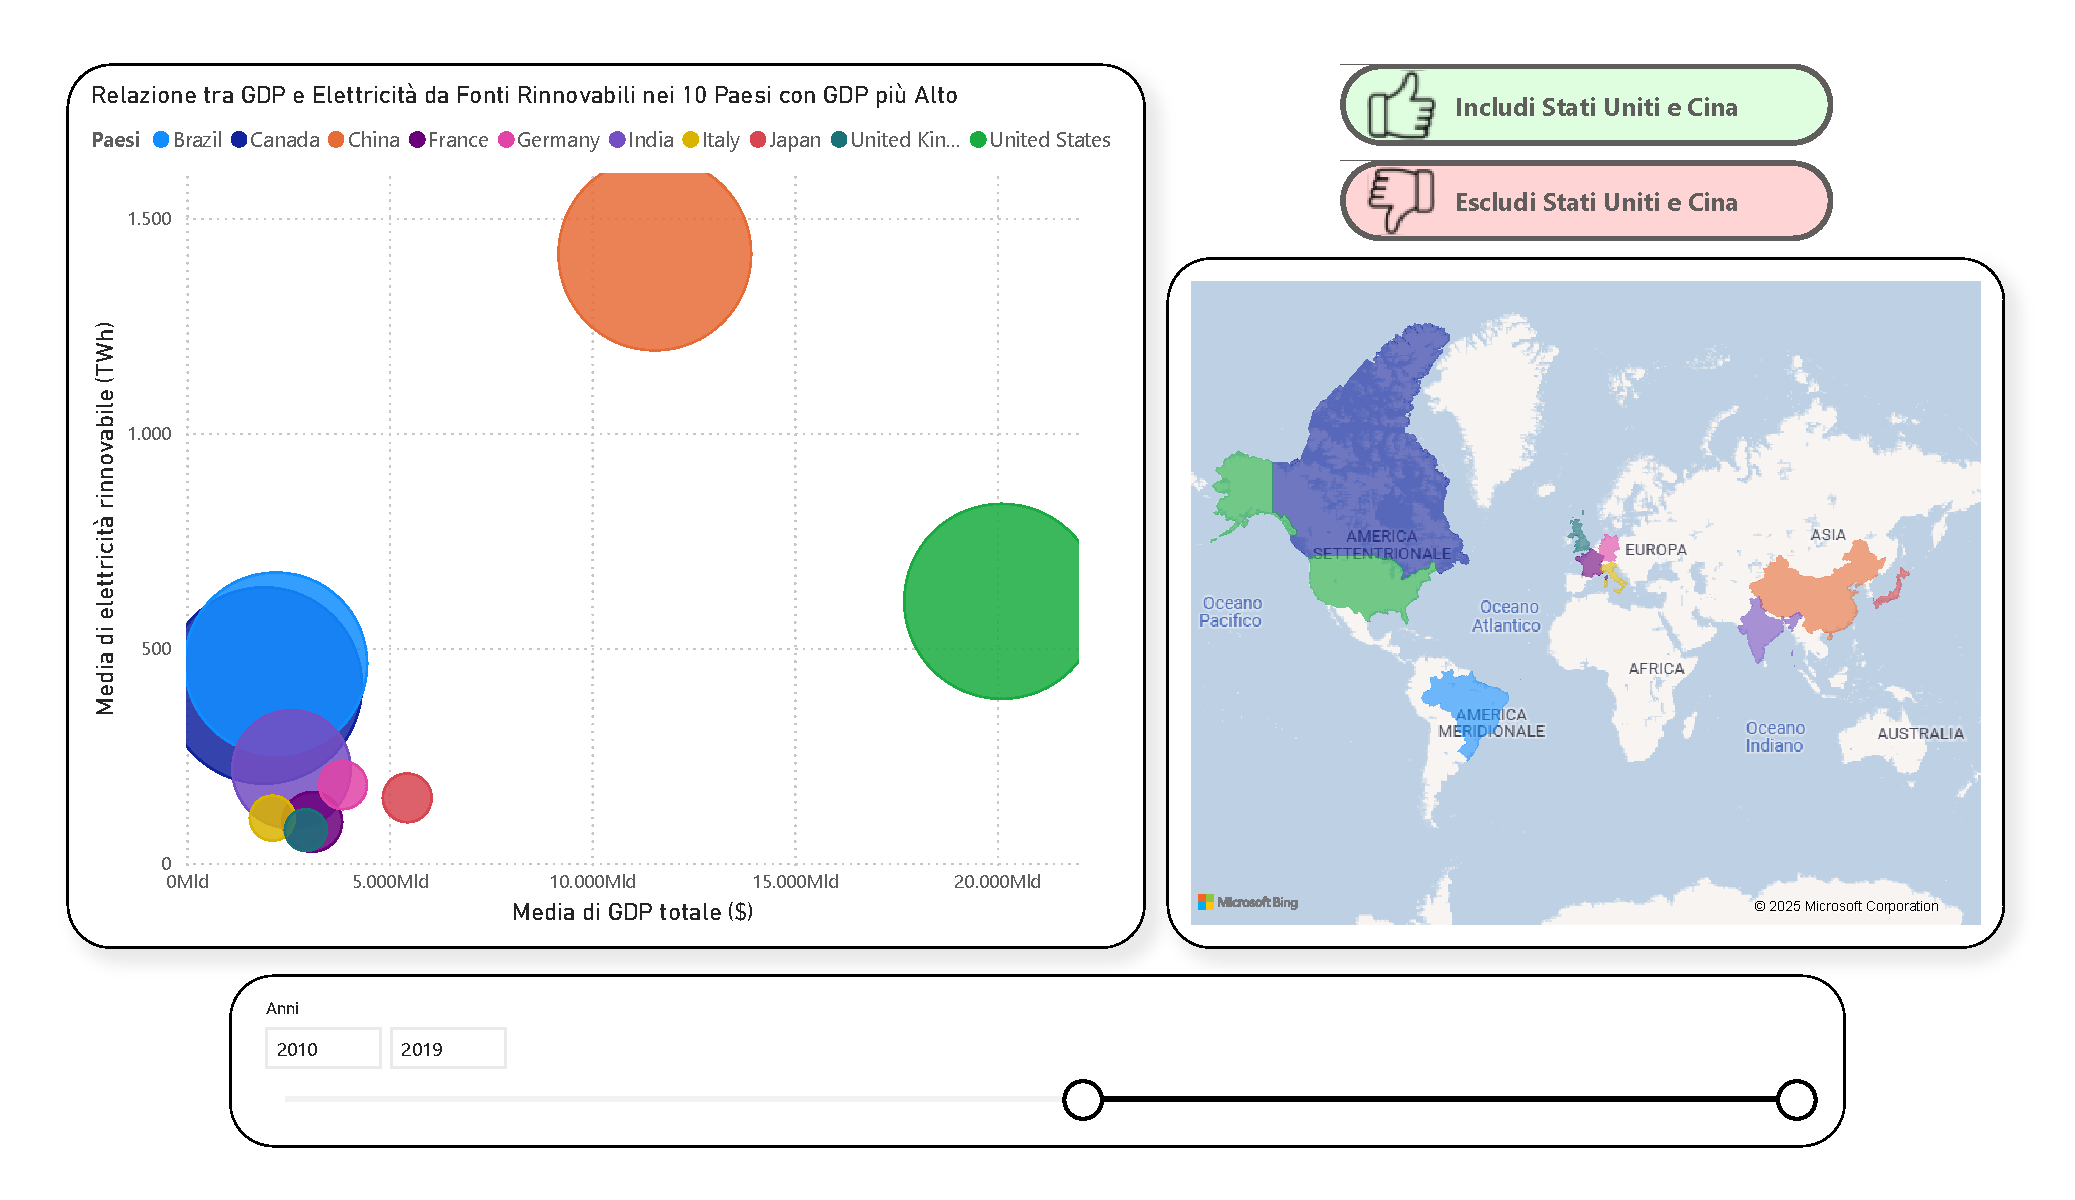
\includegraphics[width=0.9\textwidth]{capitolo_4/img4.1/Rinnovabile_GDP_2010_2019_conCinaeUSA.pdf}}\\
    \subfloat[\textbf{Risultati senza USA e Cina}]{%
        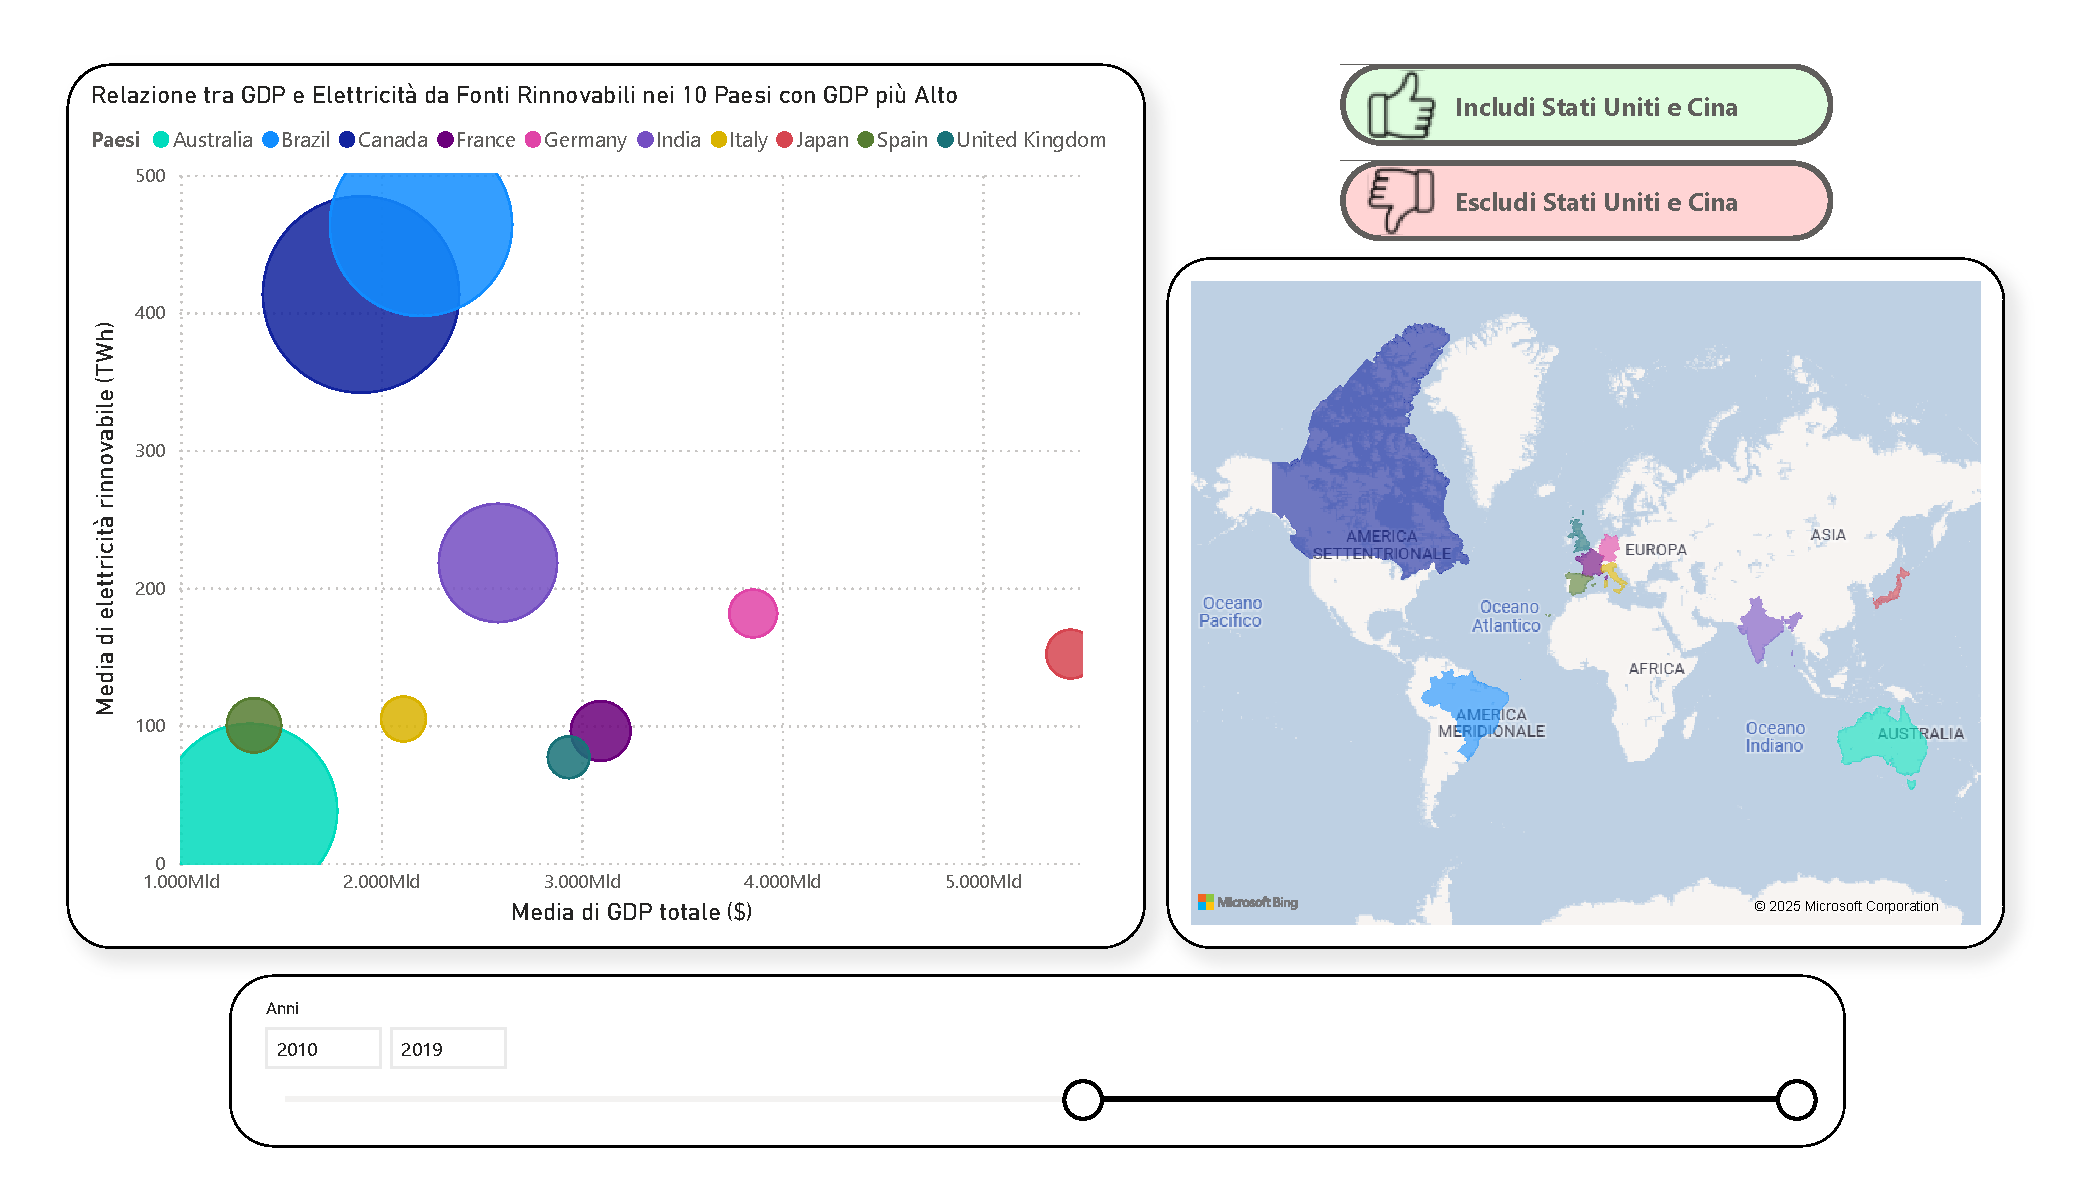
\includegraphics[width=0.9\textwidth]{capitolo_4/img4.1/Rinnovabile_GDP_2010_2019_senzaCinaeUSA.pdf}}
   \caption{Andamento della produzione di energia rinnovabile rispetto alla crescita del GDP - Anni 2010-2019}
  \label{disp_2_rinn}
\end{figure}

Dall'analisi della rappresentazione grafica emerge con chiarezza che non sussiste una correlazione diretta e lineare tra il livello di ricchezza economica di un Paese e la produzione media di energia da fonti rinnovabili. Questo risultato suggerisce che lo sviluppo economico, di per sé, non costituisce un indicatore sufficiente per prevedere l'impegno di una nazione nella transizione energetica verso fonti sostenibili.

L'impiego di energia rinnovabile appare invece fortemente influenzato da fattori di natura normativa e politico-strategica, in particolare dalle politiche ambientali adottate a livello nazionale e internazionale, nonché dagli incentivi pubblici e dalle scelte infrastrutturali orientate alla sostenibilità. Tali elementi giocano un ruolo determinante nel favorire l'adozione di tecnologie pulite e nel promuovere un modello energetico più verde.

Confrontando questi risultati con le analisi precedenti, emerge inoltre un ulteriore elemento critico: in diversi casi, pur in presenza di un aumento significativo nella produzione di energia rinnovabile, i livelli di emissioni di anidride carbonica rimangono comunque elevati. Questo fenomeno potrebbe essere attribuito alla coesistenza di fonti energetiche tradizionali ancora fortemente utilizzate, a una domanda energetica complessiva in crescita, oppure a settori industriali che non hanno ancora completato la transizione verso soluzioni a basse emissioni.






